\documentclass[a4paper, 12pt, envcountsect, runningheads]{llncs}
\usepackage{amsmath, amsfonts, url, amssymb, graphics} 
\usepackage{graphicx, color}
\pagestyle{plain}
\setcounter{page}{1}

\newcommand{\F}{{\mathbb F}}
\newcommand{\Q}{\mathbb{Q}}
\newcommand{\Z}{\mathbb{Z}}
\newcommand{\Qbar}{\overline{\Q}}
\newcommand{\Fbar}{\overline{\F}}
\newcommand{\N}{\mathbb{N}}
\newcommand{\abs}[1]{\lvert #1 \rvert}
\DeclareMathOperator{\Jac}{Jac}
\DeclareMathOperator{\charr}{char}
\DeclareMathOperator{\ord}{ord}
\DeclareMathOperator{\Aut}{Aut}
\DeclareMathOperator{\Res}{Res}

\numberwithin{figure}{section}
\numberwithin{equation}{section}
\begin{document}
\title{A note on the behaviour of the NFS in the medium prime case: Smoothness of Norms}

\author{Naomi Benger\inst{1}
\and Manuel Charlemagne\inst{2}\thanks{Founded by the National Natural Science Foundation of China (Grant 61133014) and the State Key Laboratory of Mathematical Engineering and Advanced Computing.}
\and Kefei Chen\inst{3}}
\institute{
University of Adelaide, Australia\\
\email {naomi.benger@adelaide.edu.au}\and
Shanghai Jiao Tong University, China\\
\email{charlem@sjtu.edu.cn}\and
Hangzhou Normal University, China\\
\email {chen-kf@cs.sjtu.edu.cn}}

\maketitle
\begin{abstract}
During an ongoing examination of the behaviour, in practice, of the Number Field Sieve (NFS) in the medium prime case we have noticed numerous interesting patterns. In this paper we present findings on run-time observations of an aspect of the sieving stage. The contributions of these observations to the computational mathematics community are twofold: firstly, they bring us a step closer to understanding the true practical effectiveness of the algorithm and secondly, they enabled the development of a test for the effectiveness of the polynomials used in the NFS. The results of this work are of particular interest to cryptographers: the run-time of the NFS determines directly the security level of some discrete logarithm problem based protocols, such as those arising in pairing-based cryptography.
\end{abstract}
%================================================================
\section{Introduction and Motivation}
In cryptography the {\em computational} behaviour of particular algorithms is used to determine the security level of a protocol. More specifically, as the security of cryptographic protocols is based on the hardness of underlying mathematical problems, it follows that the security is reliant on the computational behaviour of solving those problems in the given implementation context. It is therefore important that we have a sound knowledge of the behaviour of the algorithms used to solve these problems in practice in order to implement cryptographic protocols with reliable security settings.

The Discrete Logarithm Problem is the basis of security in numerous cryptographic protocols instantiated in either the additive group of points on an elliptic curve (ECDLP) or a multiplicative group of a finite extension (DLP). 
The most efficient known algorithms to solve the ECDLP have been thoroughly examined and the behaviour of these algorithms in practice is well understood, for example see \cite{pollard,teske,rho_chal_1,rho_chal_2,rho_efficiency}. The DLP in medium prime extension fields has received comparably less attention, so the understanding of the behaviour of the algorithm to solve it is limited. The result of this is that we are not able to give precise implementation guidelines for protocols with security dependent on the hardness of this DLP instance. In particular, in Pairing-Based Cryptography (PBC) the underlying problems that form the basis for security are usually related to variations of both the ECDLP and DLP -- the hardness of the first problem is well understood but hardness of the second still remains elusive; this complicates parameter selection.


There are various known algorithms for solving the DLP, the most appropriate depends on the context of the problem. According to the complexity analysis in \cite{joux-lercier-smart-vercauteren06}, the Number Field Sieve (NFS) in the medium prime case is the most efficient algorithm to solve the instances of finite field DLP occurring in PBC; these instances are in the ``small prime'' category \cite[Section 3.1]{joux-lercier-smart-vercauteren06}. 

Little is known about the practical effectiveness of the NFS in the medium prime case which limits our understanding of the security of PBC protocols. In this work we examine one aspect of this NFS version.

The ultimate goal of this continuing project is to increase the general understanding of the behaviour of the NFS. The motivation for this work is threefold: firstly, the behaviour of other NFS versions is known to vary widely \cite{zajac,dan_predicting_nfs}. Secondly, implementation of cryptographic protocols on small devices requires accurate security estimates as memory and processing power are limited. Finally, recent advances in solving the DLP in binary fields \cite{FFS_rob, FFS_antoine, joux_imporved} will promote the use of medium prime fields in PBC, over binary fields; it is necessary to investigate the problem in this increasingly utilised setting.


The analysis of the NFS algorithm in \cite{joux-lercier-smart-vercauteren06} is given for finite fields $\F_{p^k}$ as both $p$ and $k$ tend to infinity which necessitates loss of detail and generalisation to limiting cases. We wish to fine-tune this analysis, model the behaviour of the NFS in the context of  cryptography, retaining as much detail as possible, performing statistical analysis on experimental results. In this work we outline some of the practical observations made during our analysis. Using these observations we have developed a ``pre-NFS'' polynomial test on the effectiveness of a particular NFS instance. We also introduce a variation in the NFS polynomial selection. The results of our work will be of interest to implementers of the NFS and pairing-based protocols alike. 
The remainder of this paper is organised as follows: In section \ref{s:nfs} we give a brief introduction to the NFS. In section \ref{s:smooth} we examine one aspect of the theoretical complexity analysis, which solidifies our motivation and introduce the particular aspect of the NFS that this work focuses on. In section \ref{s:context} we explain our experiment setting and the process of our investigation, presenting the results of this undertaking in section \ref{s:results}. Conclusions and open problems are presented in section \ref{s:conclusion}.
%================================================================ 
\subsection*{Acknowledgments}
The authors thank Mike Scott and Rob Granger for their continual advice and support, Nigel Bean and Jono Tuke for helpful discussions.
%================================================================

\section{NFS in a nutshell} 
\label{s:nfs}
In this section we give a brief introduction to the NFS. The NFS can be considered a sequence of stages for which we assess the complexity separately. The two main parts of the NFS are the sieving stage and the linear algebra stage, these are followed by a descent stage. Suppose we wish to solve a DLP instance in the finite field $\F_{p^n}.$

In the sieving stage we aim to construct a set of linear equations in the logarithms of ``small'' elements. This is done using two number fields, say $\mathcal{K}_{1}$ and $\mathcal{K}_{2}$, both of which contain $\F_{p^n}$ as a subfield. We sieve through the elements of these fields looking for ``doubly-smooth'' pairs. Two elements form a {\em pair} if the mappings from their respective number fields to $\F_{p^n}$ maps them to the same element. An element is {\em smooth} if it can be written as the product of {\em small} elements, elements with norms a prime number below a given bound; the pair is {\em doubly-smooth} if both are smooth in their respective number fields. 

The system of linear equations is solved in the linear algebra stage, finding the discrete logarithms of the small elements. In the descent stage the specific element of interest is written as a product of small elements and thus its discrete logarithm is found. 

In this work we examine the complexity of the sieving stage. For the NFS variation relevant to the PBC context, the two number fields are constructed as $\mathcal{K}_{i}=\Q[\theta_i]$ for $i\in\{1,2\}$. The element $\theta_i$ is a zero of the irreducible polynomial $f_i(x)$ with integer coefficients such that $n\mid\deg(f_i)$; $f_1$ and $f_2$ have a common root modulo $p$. The elements of these number fields are thus considered as polynomials of degree $t<n$ in $\theta_i$. To compute the norm of an element $a=a(\theta_i)$ in $\mathcal{K}_i$ we consider $a$ as a polynomial in $x$ and take the resultant of $a(x)$ with $f_i(x).$ To find doubly-smooth pairs we look at the factorisation of the norms of the elements.



%\subsection*{Sieving}
%\label{ss:sieving}
%The goal of the sieving stage is to find a set of linear relations in the logarithms of a fixed set of elements. This is done by selecting two isomorphic representations of a number field of dimension $k$ over $\Q$, say $\mathcal{K}_{1}$ and $\mathcal{K}_{2}$, and fixing a subset of elements in each of the representations, called the \textit{Factor Base}, denoted by $\mathcal{F}_{1}$ and $\mathcal{F}_{2}$ respectively. The factor bases contain the ideals of small norm, bounded by a {\em smoothness bound} $\mathcal{B}_{i}$, $i=[1,2]$.
%Field elements are then `sieved' to find pairs $(\alpha,\beta)$, $\alpha\in\mathcal{K}_{1}$ and $\beta\in\mathcal{K}_{2}$, with $\alpha\cong\beta$, and $\alpha$ and $\beta$ {\em smooth} over their respective factor bases; that is, $\alpha$ and $\beta$ can be completely decomposed into a product of elements from their respective factor bases. Such pairs are called \textit{doubly smooth}. The sieving continues until enough relations $$\alpha=\prod_{\gamma_{i}\in\mathcal{F}_{1}}\gamma_{i}^{a_{i}}\cong\prod_{\delta_{j}\in\mathcal{F}_{2}}\delta_{j}^{b_{j}}=\beta$$ are found, that is, at least the sum of the number of elements in the factor bases.
%These relations are converted to linear equations in the logarithms of the factor base elements by taking the discrete logarithms of each side with respect to fixed (isomorphic) elements in each representation.
%In the particular variation of the NFS we are concerned with here, the two number fields are constructed by adjoining to $\Q$ roots $\theta_1$ and $\theta_2$ of two different polynomials ($f_1$ and $f_2$ respectively, considered in $\Z[x]$) which have common root modulo $p$. The elements of these number fields are thus considered as polynomials of degree $t<n$ in $\theta_i$. To compute the norm of an element $a=a(\theta_i)$ in $\mathcal{K}_i$ we consider $a$ as a polynomial in $x$ and take the resultant of $a(x)$ with $f_i(x).$
%\subsection*{Linear Algebra}
%\label{ss:LinAlg}
%The system of linear equations obtained in the sieving stage is solved using linear algebra to find the logarithms of the elements in the factor bases.
%Solving the linear equations is no trivial task. Though the matrix of equations is originally sparse, after only a few operations it becomes congested. There are a few methods for reducing this matrix and solving for the unknown logarithms: Lanczos algorithm, Wiederman algorithm and structured Gaussian elimination  (all with complexity $\leq L(1/3)$), some algorithms use a combination of these methods \cite{lamacchia-odlyzko}. 
%================================================================
\section{Smoothness probability of norms}
\label{s:smooth}
The run time of the sieving stage of the NFS is determined by the probability of finding doubly smooth relations. There exist varying methods in the literature to predict smoothness probabilities in different contexts.
Denote by $\Psi(x,y)$ the number of integers $\leq x$ with no prime factor exceeding $y$; the probability of a random integer of size approximately the size of $x$ being {\em $y$-smooth} is $\Psi(x,y)/x.$ 
In \cite{hild-tene} a comprehensive survey of estimates for $\Psi(x,y)$ is given; in the more recent \cite{dan_psi_est} we are presented with a method for computing $\Psi$ within an arbitrarily tight bound. The results of \cite{krause} are extensions of some of the theorems in \cite{hild-tene} to the context of algebraic numbr fields -- the relevant case for the NFS. The formul{\ae} for calculating the probability is directly obtained from the $\Psi_K(x,y)$ estimate (number of integral ideals with norm $< x$, all of whose prime divisors have norm $< y$ in a number field $K$) \cite[Satz 3]{krause} but computation of this estimate is not feasible in practice and therefore can not be used in the complexity analysis of the NFS algorithm. The computation relies on knowledge of the class number of $K$ and a result of the Dedekind Zeta function, both of which are known to be hard to compute in practice.
This presents a major set back when trying to estimate the computational behaviour of the NFS: we are unable to compare the behaviour of an NFS instance to the estimate. Indeed, the variability of the probability of smoothness of norms in given number fields (that is, for a given choice of $f_1$ and $f_2$) could be used to explain some of the behaviour noticed by Zajac \cite{zajac}; thus the ability to compute this probability would aid polynomial selection. 
The smoothness probability estimate for integers used for the complexity analysis in \cite{joux-lercier-smart-vercauteren06} is from a corollary \cite[page 15]{can-er-pom}; this formula is the most appropriate choice, given that the algorithm is presented for extension degrees $k$ and primes $p$ both tending to infinity. 

%================================================================
\section{Analysis Context}
\label{s:context}
In this section we outline our experiment parameters and a variation of the NFS polynomial selection process. 
\subsection*{Parameter sizes}
As the contextual focus is PBC, we used the current field size suggestions in literature (from resources such as \cite{lenstra-verheul,lenstra01,ECRYPT_key_sizes}) for the security levels 80, 128 and 192 which fixes the types of elliptic curves which can be used and therefore also fixes $n$. We used the complexity analysis of \cite{joux-lercier-smart-vercauteren06} to compute the corresponding values for $t$ (degree of elements sieved) for each of the 3 instances. That gives us:
\begin{center}
\begin{tabular}{|c|c|c|c|}
\hline
&80 bit security & 128 bit security & 192 bit security\\
\hline
curve & MNT6 & BN & KSS18\\
size of $p$ & 160 & 256 & 512\\
$n$ & 6 & 12 & 18\\
$t$ & 2 & 3-4 & 4\\
\hline
\end{tabular}
\end{center}
We present our results using a working example of the MNT6 case; the methods are directly adaptable to the BN and KSS18 cases. 
\subsection{Polynomial selection}
\label{ss:poly_selection}
In order to have the NFS polynomials of simple structure, we find two numbers $a_1,\;a_2$ of size $\sim\sqrt{p}$ of such that $a_1\cdot a_2=p+i$, where $i$ is some small integer. We define the polynomials $f_1$ and $f_2$:
\begin{eqnarray*}
f_1 &=& x^n + a_2\\
f_2 &=& a_1 x^n + i
\end{eqnarray*}
when both are irreducible. It is straightforward to show that these polynomials have a common zero modulo $p$ (in fact have the same set of zeros) and are therefore appropriate for use in the NFS. Using this polynomial selection means that the sieving space did not need to be skewed to balance the sizes of the norms of the elements in each number field (see \cite{joux-lercier-smart-vercauteren06} for details). One important detail supporting the use of binomials in this context is that for efficient pairing implementation the prime is chosen to be $p\equiv1\mod n$ (or the prime factors of $n$) \cite{koblitz-menezes05}, thus it is possible to find irreducible binomials for the NFS polynomial selection in this context. (For the BN case we were able to use irreducible polynomials as used for the tower constructions in \cite{towers}.) %Initial results showed that this new method is more likely to find smooth elements than the original polynomial selection; the reasons for this are still yet to be thoroughly investigated.
%================================================================
\section{Norm Smoothness Analysis}
\label{s:results}
In this section we present our methodology and the results of our work; the process is divided into three sections:
\begin{itemize}
\item[\ref{ss:norms_dist}] We used empirical data to compute the cumulative distribution function of the norms; we make observations about which parameters influence the distribution; we illustrate how the cumulative distribution affects the smoothness probability.

\item[\ref{ss:smoothness}] We show how to compute an improved estimate of the smoothness probability using the cumulative distribution function and the results of \cite{dan_psi_est}.

\item[\ref{ss:poly_test}] We present a test for the effectiveness of the $f_1$ and $f_2$ polynomials against the expected outcome.

\end{itemize}
\subsection{Cumulative Distribution of Norms}
\label{ss:norms_dist}
Once the polynomials $f_1$ and $f_2$ have been selected, the computation of the norms can be reduced to the evaluation of a polynomial in the coefficients of the number field elements. The coefficients are taken from a fixed interval $[0,S]$ for a sieving bound $S$, computed following the instructions in \cite{joux-lercier-smart-vercauteren06}, as is the smoothness bound $\mathcal{B}$. We can therefore consider the coefficients as independent random variables $X_0,\ldots,X_t$ randomly selected from $[0,S]$ following a uniform distribution. The norm is also a random variable, $N$, which takes values in the range of the function on the random variables $X_0,\ldots,X_t$ defined by the determinant of the Sylvester matrix; we denote this function $n(X_0,\ldots,X_t)$. We are interested in the cumulative distribution of $N=n$. 
%The smoothness probability looks at the \textit{size} of integers as opposed to the actual integer, so we are interested in the distribution of the size of the norm, that is $z=log(s(x_0,\ldots,x_t))$ for particular values $X_i=x_i$. The values taken by $z$ are modelled by the continuous random variable $Z$, what remains is to find the distribution of $Z$. For this we use the method of distribution functions on random variables.
The reason for focussing on the cumulative distribution is that the estimates for the probability of smoothness are in fact cumulative probabilities: $\Psi(x,y)/x$ where $\Psi(x,y)$ is the number of integers $\leq x$ with no prime factor exceeding $y$. We will use the cumulative distribution of $N$ to weight the smoothness probability estimate of the integers to find a more appropriate smoothness probability estimate for the norms.
The resultant of polynomials of the form $Ax^6+B$ with $X_0+X_1 x +X_2 x^2$ (the MNT6 setting) is given by the evaluation of the function {\small{$$n(X_0,X_1,X_2,X_3)=A^2 X_0^6 - 2 A B X_0^3 X_2^3 + 9 A B X_0^2 X_1^2 X_2^2 - 6 A B X_0 X_1^4 X_2 + ABX_1^6 + B^2 X_2^6,$$}} where $A=1$ for $f_1$. Such a number clearly has much structure and numbers generated using this equation will have a distribution very different from the uniform, which is used in the complexity analysis. Trialling various theoretical methods to determine the probability distribution of this $N$ from this function of uniform random variables was unfruitful due to the complexity and large number of variables. We therefore generated empirical data to directly determine the cumulative distribution. 
In the following graph we see the cumulative distribution function as generated for the norms for the MNT6 case. Intuitively, we expect a ``clumping'' effect in the centre of the probability distribution of the norms due to the fact that we are repeatedly summing 6th powers of uniform variables from a bounded interval, which will increase the proportion (and therefore probability) of the low to middle range norm values. The result of this clumping effect in the probability distribution translates to a very steep cumulative distribution function over the low and middle range (plentiful) values, which tapers down to very small slope over the larger (rarer) values. This is exactly the result that the data presented. In figure \ref{fig:comp} we see the cumulative distribution function as generated for the norms for the MNT6 case compared with the uniformly distributed variable.
It is clear that this central clumping as discussed above results in the ``mid-range'' values being more probable in the norm distribution than for the integers: The number of integers in a particular interval increases constantly with the upper bound of the interval whereas the norms have a higher concentration in the mid-range of the same interval, a direct result of the range of the variables $X_0,X_1,X_2$. 
%\begin{center}
\begin{figure}\label{fig:comp}
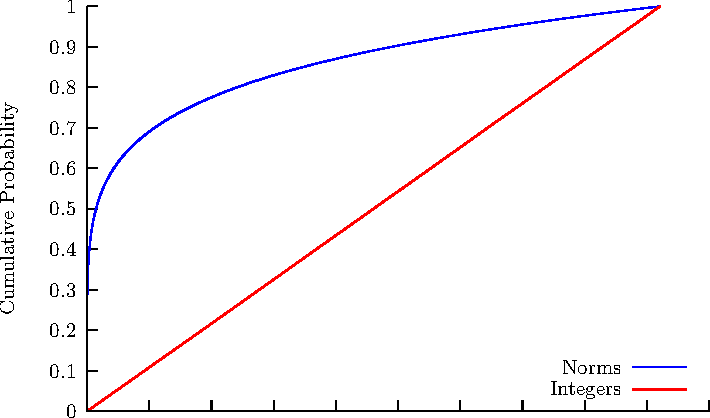
\includegraphics[scale=1]{graphs/cumulative}\caption{Comparison of the cumulative distribution of norms and uniform integers in the MNT6 case. This particular graph generated using $p=1125909838976401$ ($s=349879$).}
\end{figure}
%\end{center}
Another interesting observation we made, by varying the size of $p$ for more tests, is that the distribution of the norms depends only on $k$ and $t$. The size of $p$ only dictates the \textit{placement} of the distribution %, as it directly determines the interval from which the variables $X_0,X_1,X_2$ are taken, 
not the \textit{shape}. This is not surprising given that the shape of the elements of interest are the output of the above function $n(X_0,\ldots,X_t)$, a degree $k$ function in $t$ variables, with constants $A$ and $B$ being altered with each function. For this reason we use a smaller example case than would be used in practice: the MNT6 setting and a 50-bit prime (with $k=6$ and $t=2$). This allows us to perform more thorough and varied tests. We recalculated the sieving bound to correspond with the new field size, following the instructions in \cite{joux-lercier-smart-vercauteren06}, but preserved the value for $t$.


\subsubsection*{Fitting a line to the cumulative distribution}
The line which depicts the cumulative distribution as presented in figure \ref{fig:comp} was generated using 2 million norm values ($X_0,X_1,X_2$ chosen uniformly at random) for a range of primes and polynomials, with negligible variance. To obtain the equation of this line we performed curve fitting using R, a language package for statistical computing \cite{R}. Initial experiments indicated that this is not an exponential curve prompted us to use the {\em Box-Cox method} \cite{box-cox}. This method aids us in identifying a suitable power transformation on the response variable ($y=$ the proportion of norm values $\leq x$) to obtain a linear relationship between the explanatory variable ($x$) and the modified response variable; that is, we wish to find a value $\lambda$ such that $y^\lambda=ax+b$. Often the initial test range for $\lambda$ is $[-5,5]$ and the default setting in R is $[-2,2]$ incrementing in steps of $0.1$. The graph in fig \ref{fig:comp} represents the density of norm values and as the norms are sums of monomials of degree 6 we expect $\lambda$ to be close to 6 and therefore set our test range to be $[0,10]$. Instead of using all 2 million points (which would have made the tests very slow) we repeated the test numerous times on random samples of 10000 points. The results for each of the tests gave clear indication that $\lambda=6$ (see appendix \ref{A:diagrams}). 
We then proceed to fit a linear model to the full data set of points of the transformed data $(x,y^6)$ to find that $Y^6=aX+b$ where $a=2.171E-106$ and $b=-1.868E-5$. From a statistical perspective the fit is incredibly accurate as there is no noise in the data, given the smoothness of the curve generated from our empirical values we expect to have little error. Exact output of the linear model fitted in R is given in appendix \ref{A:diagrams}


\subsubsection*{How the cumulative distribution affects the smoothness probability}
To illustrate why the probability of smoothness is affected by the differing probability distributions we use the law of total probability. Let us examine the problem in terms of random variables: Let $Z$ be a random variable which takes integer values (without loss of generality we assume that the interval is $[0,U]$ for some bound $U$). Let $N$ be a randomly selected norm (also from the interval $[0,U]$) and let $S_Z$ (resp. $S_N$) be a binomial random variable such that 
\begin{equation}
S_Z=\left\{\begin{array}{ll}
1 & \mbox{if }Z=z\mbox{ is smooth};\\
0 & \mbox{if }Z=z\mbox{ is not smooth}.
\end{array}\right.
\end{equation}
We define $S_N$ similarly where smooth in both cases is with respect to some fixed bound $\mathcal{S}$. Now the probability that a random integer ($z$) selected from the defined interval uniformly at random is smooth is expressed as $$P(S_Z=1| Z=z).$$ Following the law of total probability we partition the interval $[0,U]$ into $s$ equally sized sections, of width $U/s=a$, we can now write this probability as a summation: $$P(S_Z=1)=\sum_{i=1}^{s}P(S_Z=1| z\in[(i-1)a,ia])P(z\in[(i-1)a,ia]).$$ Using the same method we can rewrite $P(S_N=1)$: $$P(S_N=1)=\sum_{i=1}^{s}P(S_N=1| n\in[(i-1)a,ia])P(n\in[(i-1)a,ia]).$$
Assuming initially that the probability of a norm being smooth is equal to the probability of an integer of the same size being smooth\footnote{The validity of this assumption will be discussed further in section \ref{ss:smoothness}.} the left probability value in each of the summations will be identical for every value of $i$ and can be computed using the method of \cite{dan_psi_est} (a free implementation is available at \cite{dan_imp} courtesy of the author). From the different distributions of the norms and integers we know that the right hand values are quite different and so the sums will clearly not be equal. 
The probabilities on the right in the $P(S_Z=1)$ expression are exactly the $s$-quantiles ($s$ is the number of partitions); as $P(Z\leq ia)=\frac{ia}{U}$ and so for all $i$ we have: $$P(z\in[(i-1)a,ia])=P(Z\leq ia)-P(Z\leq (i-1)a)=\frac{(i-1)a-ia}{U}=\frac{a}{U}.$$ That is, the right probabilities in the $P(S_Z=1)$ expression are constant and the expression becomes 
\begin{eqnarray*}
P(S_Z=1)&=&\frac{a}{U}\sum_{i=1}^{n}P(S_Z=1| z\in[(i-1)a,ia])\\
&=&\frac{a}{U}\sum_{i=1}^{n}\frac{\#\mbox{smooth}\in[(i-1)a,ia]}{a}\\
&=&\Psi(\mathcal{S},U)/U.
\end{eqnarray*}
Examining figure \ref{fig:comp} we see that the probabilities $P(n\in[(i-1)a,ia])$ will be quite different. Using the law of total probability we not only highlight how the distribution of the norms affects the probability of smoothness, but present a method for computing a better estimate for the smoothness probability for the norms. 

\subsection{Estimating the smoothness probability of norms}
\label{ss:smoothness}
To compute $P(S_N=1)$ we use the same approach as above, this alters the position of the partitions used; instead of having the partitions evenly spaced (as above) we use the $s$-quantiles of the distribution of the norms (that is, we fix the intervals such that the probability that $n$ is in any interval is fixed at $\frac{1}{s}$). Fixed probability and even spacing are synonymous for the uniform distribution, but not for the distribution of the norms. Using R we easily compute the $100$-quantiles of the norms, that is, we find the values $a_0,\ldots,a_{100}$, given in appendix \ref{A:MNT100quantiles}, such that $P(n\in[a_i,a_{i+1}])=0.01$ for $i\in[0,99]$. It remains now, following from our assumption that $P(S_N=1| n\in[a_i,a_{i+1}])=P(S_Z=1| z\in[a_i,a_{i+1}])$, to compute $$0.01\sum_{i=0}^{99}P(S_N=1| n\in[a_i,a_{i+1}])$$ to have the probability of smoothness of the norms. Using the implementation \cite{dan_imp} we computed the probabilities in the summation to obtain an estimate of the smoothness probability: $$P(S_N=1)=0.0001699201=\hat{r}\;\;\mbox{ compared to }\;\;P(S_Z=1)=0.00005777868.$$
The probability of smoothness of the norms is higher by a factor of almost 3 (2.94). This is no surprise as, intuitively, smaller numbers are more likely to be smooth and the norms have a higher concentration of `small' numbers than the integers do. These results also reflect the experimental results obtained by selecting integers at random, following the distribution of the norms, and testing for smoothness; almost 3 times as many smooth integers were obtained using this method compared to selecting integers uniformly at random.

The probability above is an {\em optimistic-case} probability; we have made the assumption that the probability of a norm being smooth is equal to the probability that an integer of the same size is smooth. That is, for some integers $b_0$ and $b_1$ we assumed that $$P(S_N=1| n\in[b_0,b_1])=P(S_Z=1| z\in[b_0,b_1]).$$ This is, however, not necessarily the case. In any given interval, the integers are denser than norm values (approximately $1/6$ for the MNT6 case), and the norms will not necessarily coincide with the same proportion of smooth integers; the norms may coincide with a lesser proportion of smooth integers. On the other hand, the norms may in fact fall on more smooth integers than the ratio of integers to norms in that interval; it is in this scenario that the NFS sieving stage will execute faster. In the following table are examples of polynomials found for an example MNT6 prime for which the calculated rate $r_1$ (from $1000/\hat{r}\approx5$mil tests).\\
\newpage
$p=1125909838976401$
\begin{center}
\begin{tabular}{l|ccc}
polynomial & \# smooth & $r=$ smooth rate & $\beta=$factor difference from $\hat{r}$\\
\hline
$f=35374332x^6+11$ &633&0.0001266&0.7451\\
&&&\\
$f=11791444x^6+11$ &1370&0.0002740&1.6125\\
&&&\\
$f=17687166x^6+11$ &652&0.0001304&0.7674\\
&&&\\
$f=x^6+8264689$ &1379&0.0002758&1.6231\\
&&&\\
$f=1069214x^6+37$ &1320&0.0002640&1.5537
\end{tabular}
\end{center}
\vspace{0.5cm}
The values of $\beta$ in the fourth column can be compared with the value $0.33\hat{3}$ which is used in the complexity analysis. We see the second, fourth and fifth polynomials produce smooth norms at a rate over \%50 faster than the prediction (and so $4.5$ times the estimate used in the complexity analysis). There are, in fact, numerous polynomials for which the rate of smooth norm collection is higher than the predicted rate and we were able to find many examples, though the average case differs from $\hat{r}$ by a factor of $0.5526999$ (i.e. the mean value of $\beta$) shown in Figure \ref{fig:mults}. The long tail of the graph distorts the standard deviation, but examining the quantiles, half of the values are between $0.28$ and $0.71$ with $1$ being near the end of the main peak which is why we use the term {\em optimistic-case} probability. In figure \ref{fig:mults} the value given by the asymptotic complexity is shown and it is indeed the the value which occus with the highest probability, but it is also clear that a much larger proportion of the cases perform significantly better than this case. We see clearly now that considering only the complexity analysis in this case would lead to a misleading evaluation of the rate of smooth relation collection for a given pair of polynomials: the polynomials may exhibit smooth norms at a higher rate than the complexity analysis suggests, but still at a rate well below the average, this could lead to less efficient pairs of polynomials being selected.

The goal of an implementer of the NFS is to find a polynomial {\em pair} such that the rate of smooth relation collection in each number field is as close to $\hat{r}$ as possible: that is, we want to find pairs $(f_1,f_2)$ such that $r_1\cdot r_2\approx\hat{r}^2$ ($r_i=$ smooth rate of norms computed using $f_i$, $i\in\{1,2\}$); this is no straightforward task. We denote $r_1\cdot r_2=\delta\hat{r}^2$ and recognise that the possible values for $\delta$ will be the product of independently selected values from the distribution of $\beta$ and will therefore have mean value $\beta^2$. From our empirical data we computed $0.3320898$ very close to the predicted $0.3062898=0.5526999^2$ (graph of distribution in appendix \ref{ap:mults}). We can compare this to the estimate used in the complexity analysis which would give a value of $\delta=1/9=0.11\bar{1}$. Even if we use the median of this distribution, $0.2118865$, to remove some of the influence of the large, rare cases, it is still approximately twice the probability used in the complexity analysis and reflects more closely he observed behaviour.
%\begin{center}
\begin{figure}\label{fig:mults}
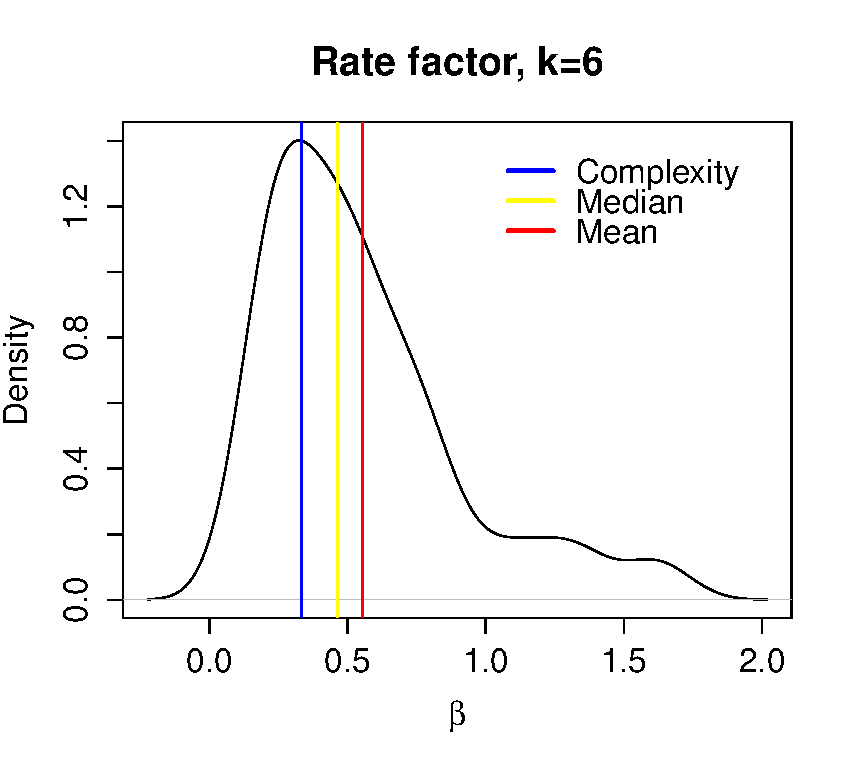
\includegraphics[scale=0.7]{graphs/multiple_tests_plot}\caption{The probability density function of the multiple by which the rate of smooth relation collection differs from the estimated rate.}
\end{figure}
%\end{center}
\subsection{Polynomial Selection Test}
\label{ss:poly_test}
The mean value of $\delta$ gives us the benchmark to aim to obtain, or improve on, when selecting our polynomials for the NFS. For a given instance of the DLP in a finite field $\F_{p^k}$ we perform the following test before launching the NFS sieving stage:
\begin{itemize}
\item[1] Compute the $\hat{r}$, the upper estimate on the smoothness probability of norms as done in section \ref{ss:smoothness}.
\item[2] Find polynomial pair $f_1$ and $f_2$ following the method given in section \ref{ss:poly_selection} or \cite{joux-lercier-smart-vercauteren06}.
\item[3] Generate $1000/\hat{r}$ \cite{dan_predicting_nfs} norm values randomly using both $f_1$ and $f_2$ and test for smoothness to approximate the rates of smooth norm occurrence for each number field.
\item[4] Compare the product of the approximate rates of smooth norms to $\hat{r}^2$: if it is ``large enough'', proceed with sieving, otherwise return to step 1.
\end{itemize}
In step 4 by large enough we want to find $\hat{\delta}\geq0.3320898$ (the mean value).

This differs to how the results in \cite{zajac} would be used, we have given a benchmark to compare the rate of smooth norm collection against, whereas previous methods would have required the generation of numerous pairs of polynomials to mutually compare the rate of smooth relation collection. Thus, our method results in fewer tests necessary to distinguish if a pair of polynomials is performing at least as well as the average case.

To illustrate, we have generated various $f_1$ and $f_2$ pairs for our example case of MNT6 with prime around 50 bits. Our experiments resulted in polynomial pairs for which smooth norms occurred at a much higher rate than others. The following tables show some example cases of polynomial pairs for MNT6 case:\\
\newpage
\noindent$p=1125909838976401$\\\\
\begin{tabular}{l|cccc}
polynomial pair & \# smooth & rate smooth & rate double smooth & $\hat{\delta}$\\
\hline
$f_1=35374332x^6+11$ &633&1.266E-4&7.54536E-9&0.2613\\
$f_2=x^6+31828441$ &298&5.96E-5&&\\
&&&&\\
$f_1=11791444x^6+11$ &1370&2.740E-4&1.17272E-8&0.4062\\
$f_2=x^6+95485323$ &214&4.28E-5&&\\
&&&&\\
$f_1=17687166x^6+11$ &652&1.304E-4&5.42464E-9&0.1879\\
$f_2=x^6+63656882$ &208&4.16E-5&&\\
&&&&\\
$f_1=x^6+8264689$ &1379&2.758E-4&1.147328E-8&0.3974\\
$f_2=136231362x^6+17$ &208&4.16E-5&&\\
&&&&\\
$f_1=1069214x^6+37$ &1320&2.64E-4&4.9632E-9&0.1719\\
$f_2=x^6+1053025717$ &94&1.88E-5&&
\end{tabular}\\\\
Interestingly, these examples highlight that simply taking a small value for $i$ ($11$ in this case) does not ensure a good polynomial pair, the rate of smooth relation collection for the first three polynomial pairs is vastly different. Though the rate is comparable in the number fields defined using the $f_2$, using the first and third pairs we found smooth relations at less than half the rate of the second pair, for which the value $\hat{\delta}=0.4062$ exceeds the mean value of $0.3320898$.\\\\
$p=1126169969103937$\\\\
\begin{tabular}{l|ccc}
polynomial pair & \# smooth & $r=$est. double smooth rate & $\hat{\delta}$\\
\hline
$f_1=x^6+4747150$ &476&1.014832E-8&0.3515\\
$f_2=237230753x^6+13$ &533&&\\
&&&\\
$f_1=x^6+186474550$ &139&6.52744E-9&0.2261\\
$f_2=6039269x^6+13$ &1174&&\\
&&&\\
$f_1=x^6+516240070$ &118&5.1212E-9&0.1774\\
$f_2=2181485x^6+13$ &1085&&\\
&&&\\
$f_1=x^6+20871667$ &202&4.7268E-9&0.1637\\
$f_2=53956877x^6+22$ &585&&\\
&&&\\
$f_1=x^6+27201934$ &251&6.68664E-9&0.2316\\
$f_2=41400364x^6+39$ &666&&\\
\end{tabular}
Again in this table we see great variation in the rate of smooth element collection in the first three cases, for which the same value $i=13$ was used to construct the polynomial pairs. For this prime the value of $\hat{\delta}=0.3515$ slightly exceeds the mean value $0.3320898$.

\section{Conclusion and Open Problems}
\label{s:conclusion}
In theoretical complexity of algorithms it is common practice that many constant factors are hidden in the $O$ and $L$ notations. As a result, the theoretical complexity does not give a good reflection of how the algorithm will run in practice.  
In cryptography, the security of protocols is directly related to the {\em practicality} of solving hard mathematical problems. Until now the practical behaviour of the number field sieve in the medium prime case has received relatively little attention. Due to its relevance to the security of pairing-based protocols in particular we are examining the run-time behaviour of this algorithm in the given context; the motivation of this work was to deepen the understanding of the NFS in general, in the hope that this would help determining more precise estimates for appropriate parameter sizes for a fixed security level for PBC protocols. 

In this work we presented some observations on the behaviour of the NFS in practice. We focussed on the smoothness probability of the norms of number field elements as it determines the practical run-time of the sieving stage. Our observations and analysis have resulted in a pre-sieving test that can be performed on the selected polynomials. This test ensures as efficient a set up and execution of the sieving stage as possible. The new revelation about the probability of smooth norm occurrence is a step towards a more precise run-time estimate of the sieving stage. We also gave a variation of the polynomial selection method given in \cite{joux-lercier-smart-vercauteren06} used to conduct our experiments, which shows promising behaviour.

This work covers the initial progress in the examination of the NFS sieving stage; in order to compute the expected run-time of this stage it remains to investigate the true cost of smoothness test (relative to computing power). Other tasks include a thorough comparison of the polynomial selection methods as given in section \ref{ss:poly_selection} and \cite{joux-lercier-smart-vercauteren06}. 


\bibliography{smoothness}
\bibliographystyle{plain}
\newpage
\appendix
\section{MNT6 output}\label{A:MNT6_output}
Diagram from Box-Cox method clearly indicating that for the MNT6 case that $\lambda=6$.\\
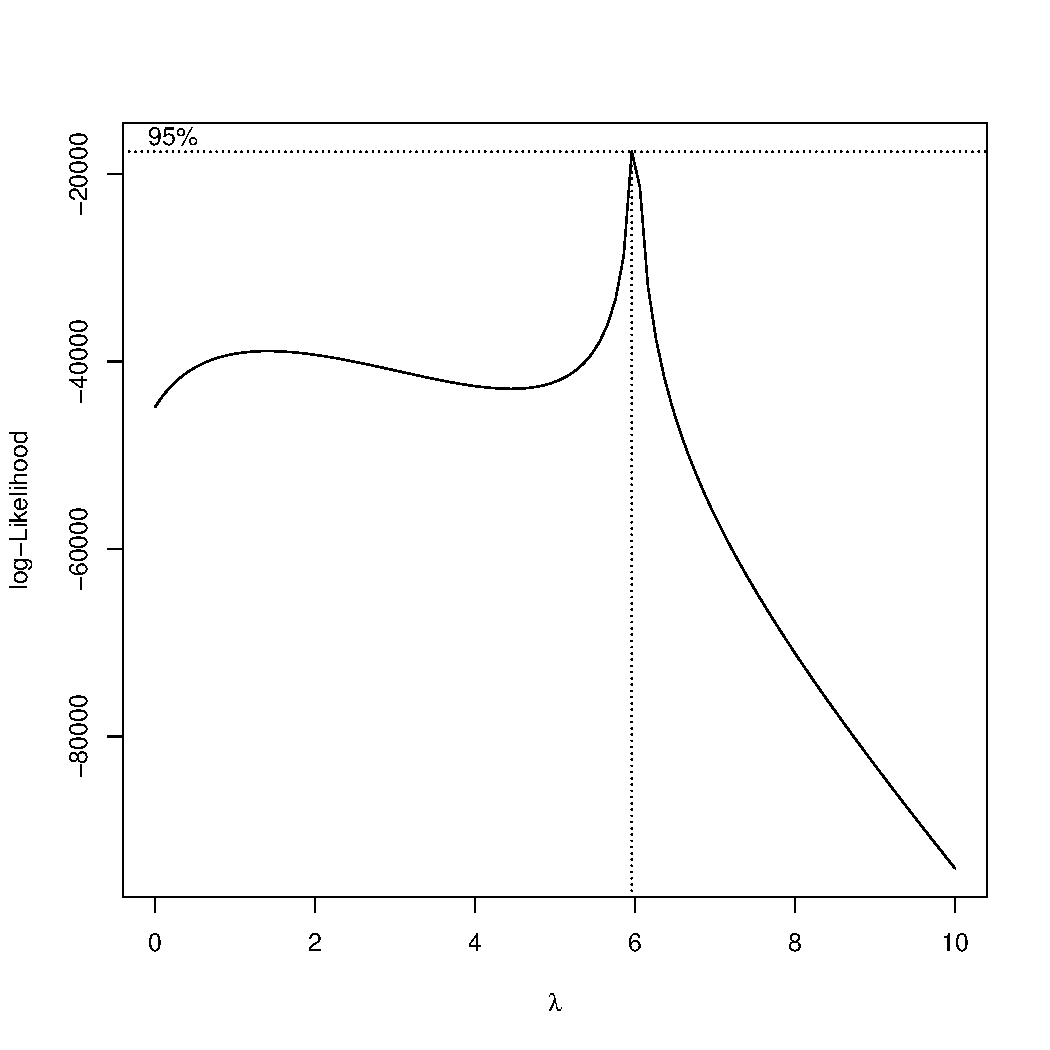
\includegraphics[scale=0.45]{graphs/CheckLineFit2}\label{fig:boxcox}\\
Comparison of the experimental data and the fitted line.\\
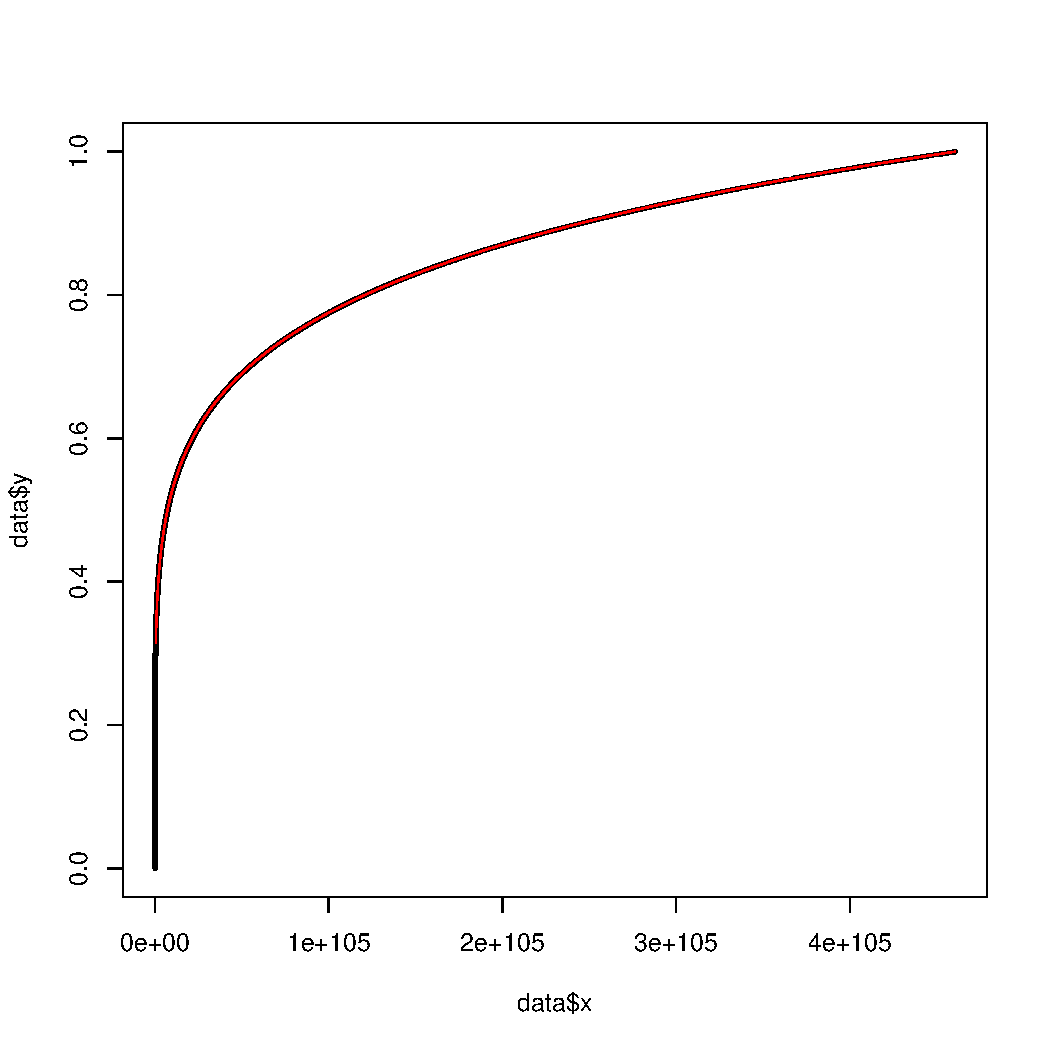
\includegraphics[scale=0.45]{graphs/CheckLineFit4}\label{fig:linefit}

\subsection{Output of the linear model}\label{A:diagrams}
Output from R:\\\\
\begin{tabular}{lcccc}
Residuals:&&&&\\
Min & 1Q & Median & 3Q & Max\\ 
-8.589e-04 & -7.149e-05 & 3.580e-06 & 1.868e-05 & 7.928e-04 \\
&&&&\\
Coefficients:&&&&\\
					& Estimate & Std. Error & t value & $Pr(>|t|)$    \\
(Intercept) & $-1.868e-05$ &  $1.701e-07$  &  $-109.8$ & $< 2e-16$\\
x          &  $2.171e-0106$ & $1.331e-112$ & $1630932.3$ & $< 2e-16$\\
\end{tabular} \\
Residual standard error: 0.0002061 on 1999998 degrees of freedom\\
Multiple R-squared:\quad 1,\quad Adjusted R-squared:\quad 1 \\
F-statistic: $2.66e+12$ on 1 and 1999998 DF,  p-value: $< 2.2e-16$


\subsection{MNT6 100-quantiles}\label{A:MNT100quantiles}
{\small{
\begin{tabular}{cccccccccc}
$a_0=$71058 &96343& 98717&100100&101069&101816&102434&103022&103837&104597\\
$a_{10}=$105289&105918&106496&107028&107524&107984&108412&108814&109192&109551\\
$a_{20}=$109893&110222&110534&110829&111113&111383&111644&111894&112137&112371\\
$a_{30}=$112596&112816&113027&113235&113434&113629&113817&114000&114180&114353\\
$a_{40}=$114522&114687&114848&115002&115154&115304&115449&115594&115735&115871\\
$a_{50}=$116004&116136&116265&116392&116517&116641&116762&116881&116997&117110\\
$a_{60}=$117221&117331&117440&117546&117650&117754&117856&117956&118055&118152\\
$a_{70}=$118249&118342&118435&118527&118618&118707&118795&118884&118971&119056\\
$a_{80}=$119140&119224&119306&119386&119465&119544&119622&119698&119775&119850\\
$a_{90}=$119925&119999& 120073& 120144& 120215& 120286&120356&120424&120493&120561\\
$a_{100}=$120628&&&&&&&&&\\
\end{tabular}
}}\\
When $N$ is a random variable which takes values from the range of the function $n(X_0,X_1,X_2,X_3)=A^2 X_0^6 - 2 A B X_0^3 X_2^3 + 9 A B X_0^2 X_1^2 X_2^2 - 6 A B X_0 X_1^4 X_2 + ABX_1^6 + B^2 X_2^6$ where $X_i$ are uniformly distributed discrete random variables in the interval $[0,349879].$ The above values are such that for $N=n$, $P(n\in[a_i,a_{i+1}])=0.01$ for $i\in[0,99]$.

%\section{Norm Formul{\ae} for other families}\label{A:other_fams}
%\subsection*{BN}
%$$f_1=x^{12}+A$$
%\begin{eqnarray*}
%&&n(X_0,X_1,X_2,X_3)\\
%&=&A^3 X_0^{12} + 3 A^2 X_0^8 X_3^4 - 48 A^2 X_0^7 X_1 X_2 X_3^3 - 24 A^2 X_0^7 X_2^3 X_3^2 + 40 A^2 X_0^6 X_1^3 X_3^3 \\
%&&+ 180 A^2 X_0^6 X_1^2 X_2^2 X_3^2 + 60 A^2 X_0^6 X_1 X_2^4 X_3 + 2 A^2 X_0^6 X_2^6 - 180 A^2 X_0^5 X_1^4 X_2 X_3^2 \\
%&&- 240 A^2 X_0^5 X_1^3 X_2^3 X_3 - 36 A^2 X_0^5 X_1^2 X_2^5 + 42 A^2 X_0^4 X_1^6 X_3^2 + 252 A^2 X_0^4 X_1^5 X_2^2 X_3 \\
%&&+ 105 A^2 X_0^4 X_1^4 X_2^4 - 96 A^2 X_0^3 X_1^7 X_2 X_3 - 112 A^2 X_0^3 X_1^6 X_2^3 + 12 A^2 X_0^2 X_1^9 X_3 \\
%&&+ 54 A^2 X_0^2 X_1^8 X_2^2 - 12 A^2 X_0 X_1^{10} X_2 + A^2 X_1^{12} + 3 A X_0^4 X_3^8 - 48 A X_0^3 X_1 X_2 X_3^7 \\
%&&+ 40 A X_0^3 X_2^3 X_3^6 - 24 A X_0^2 X_1^3 X_3^7 + 180 A X_0^2 X_1^2 X_2^2 X_3^6 - 180 A X_0^2 X_1 X_2^4 X_3^5 \\
%&&+ 42 A X_0^2 X_2^6 X_3^4 + 60 A X_0 X_1^4 X_2 X_3^6 - 240 A X_0 X_1^3 X_2^3 X_3^5 + 252 A X_0 X_1^2 X_2^5 X_3^4 \\
%&&- 96 A X_0 X_1 X_2^7 X_3^3 + 12 A X_0 X_2^9 X_3^2 + 2 A X_1^6 X_3^6 - 36 A X_1^5 X_2^2 X_3^5 + 105 A X_1^4 X_2^4 X_3^4\\
%&& - 112 A X_1^3 X_2^6 X_3^3 + 54 A X_1^2 X_2^8 X_3^2 - 12 A X_1 X_2^{10} X_3 + A X_2^{12} + X_3^{12}
%\end{eqnarray*}
%Residuals:
%       Min         1Q     Median         3Q        Max 
%-8.422e-04 -7.260e-05  3.120e-06  1.841e-05  7.863e-04 
%Coefficients:
%              Estimate  Std. Error   t value Pr(>|t|)    
%(Intercept)  -1.841e-05   2.400e-06     -7.67 1.88e-14 ***
%x            2.171e-106  1.893e-111 114690.66  < 2e-16 ***
%---
%Signif. codes:  0 ?***? 0.001 ?**? 0.01 ?*? 0.05 ?.? 0.1 ? ? 1 
%Residual standard error: 0.0002063 on 9998 degrees of freedom
%Multiple R-squared:     1,	Adjusted R-squared:     1 
%F-statistic: 1.315e+10 on 1 and 9998 DF,  p-value: < 2.2e-16 
%\subsection*{KSS18}
%$n(X_0,X_1,X_2,X_3,X_4)$ too large to print here, the authors are happy to provide the equation apon request.
%&&A*X_3^18 + A^3*X_1^18 + A^2*X_2^18 + X_4^18 - A^4*X_0^17*X_1 + 3*A*X_1^6*X_4^12 - 2*A*X_2^9*X_4^9 - A^3*X_0^9*X_2^9 + 2*A^2*X_0^6*X_3^12 + A^3*X_0^12*X_3^6 + A^2*X_0^9*X_4^9 - 2*A^2*X_1^9*X_3^9 + 3*A^2*X_1^12*X_4^6 - 18*A*X_2*X_3^16*X_4 - 14*A^3*X_0^2*X_1^13*X_2^3 + 120*A^3*X_0^2*X_1^14*X_2^2 + 78*A^3*X_0^3*X_1^11*X_2^4 - 455*A^3*X_0^3*X_1^12*X_2^3 - 220*A^3*X_0^4*X_1^9*X_2^5 + 1001*A^3*X_0^4*X_1^10*X_2^4 + 330*A^3*X_0^5*X_1^7*X_2^6 - 1287*A^3*X_0^5*X_1^8*X_2^5 - 252*A^3*X_0^6*X_1^5*X_2^7 + 924*A^3*X_0^6*X_1^6*X_2^6 + 84*A^3*X_0^7*X_1^3*X_2^8 - 330*A^3*X_0^7*X_1^4*X_2^7 + 45*A^3*X_0^8*X_1^2*X_2^8 + 56*A^2*X_0^2*X_1^6*X_3^10 - 15*A^2*X_0^3*X_1^4*X_3^11 - 70*A^2*X_0^4*X_1^3*X_3^11 - 12*A^3*X_0^3*X_1^13*X_3^2 + 91*A^3*X_0^4*X_1^12*X_3^2 - 44*A^3*X_0^5*X_1^10*X_3^3 + 220*A^3*X_0^6*X_1^9*X_3^3 - 48*A^3*X_0^7*X_1^7*X_3^4 + 210*A^3*X_0^8*X_1^6*X_3^4 + 56*A^3*X_0^10*X_1^3*X_3^5 - 2*A^2*X_0^2*X_1^9*X_4^7 - 12*A^2*X_0^2*X_2^11*X_3^5 + 104*A^2*X_0^2*X_2^12*X_3^4 + 135*A^2*X_0^3*X_1^8*X_4^7 - 45*A^2*X_0^3*X_2^8*X_3^7 + 275*A^2*X_0^3*X_2^9*X_3^6 - 56*A^2*X_0^4*X_2^5*X_3^9 + 294*A^2*X_0^4*X_2^6*X_3^8 + 18*A^2*X_0^5*X_1^5*X_4^8 - 15*A^2*X_0^5*X_2^2*X_3^11 + 91*A^2*X_0^5*X_2^3*X_3^10 + 180*A^2*X_0^6*X_1^4*X_4^8 - 21*A^3*X_0^5*X_1^11*X_4^2 + 66*A^3*X_0^6*X_1^10*X_4^2 + 48*A^3*X_0^8*X_1^7*X_4^3 - 84*A^3*X_0^9*X_1^6*X_4^3 - 56*A^3*X_0^10*X_2^5*X_3^3 + 28*A^3*X_0^10*X_2^6*X_3^2 - 10*A^3*X_0^11*X_1^3*X_4^4 + 21*A^3*X_0^11*X_2^2*X_3^5 - 35*A^3*X_0^11*X_2^3*X_3^4 + 15*A^3*X_0^12*X_1^2*X_4^4 + 120*A^2*X_0^2*X_2^14*X_4^2 - 455*A^2*X_0^3*X_2^12*X_4^3 + 1001*A^2*X_0^4*X_2^10*X_4^4 - 1287*A^2*X_0^5*X_2^8*X_4^5 + 924*A^2*X_0^6*X_2^6*X_4^6 - 330*A^2*X_0^7*X_2^4*X_4^7 + 45*A^2*X_0^8*X_2^2*X_4^8 + 135*A^2*X_1^2*X_2^14*X_3^2 - 546*A^2*X_1^3*X_2^12*X_3^3 + 1287*A^2*X_1^4*X_2^10*X_3^4 - 1782*A^2*X_1^5*X_2^8*X_3^5 + 1386*A^2*X_1^6*X_2^6*X_3^6 - 540*A^2*X_1^7*X_2^4*X_3^7 + 81*A^2*X_1^8*X_2^2*X_3^8 - 21*A^3*X_0^11*X_2^5*X_4^2 + 20*A^3*X_0^12*X_2^3*X_4^3 - 99*A^2*X_0^7*X_3^7*X_4^4 + 99*A^2*X_0^7*X_3^8*X_4^3 - 60*A^2*X_0^8*X_3^3*X_4^7 + 150*A^2*X_0^8*X_3^4*X_4^6 + 117*A^2*X_1^4*X_2^12*X_4^2 + 330*A^2*X_1^6*X_2^9*X_4^3 + 378*A^2*X_1^8*X_2^6*X_4^4 + 126*A^2*X_1^10*X_2^3*X_4^5 - 10*A^3*X_0^13*X_3^2*X_4^3 + 63*A^2*X_1^10*X_3^6*X_4^2 - 90*A^2*X_1^11*X_3^3*X_4^4 - 17*A^3*X_0*X_1^16*X_2 - A^3*X_0*X_1^16*X_3 + 17*A*X_0*X_2^7*X_4^10 - 14*A*X_0^4*X_2*X_4^13 - 17*A^2*X_0*X_2^16*X_4 - 18*A^2*X_1*X_2^16*X_3 + A*X_0*X_3^13*X_4^4 - 17*A*X_0*X_3^14*X_4^3 - 4*A*X_0^4*X_3*X_4^13 + 18*A*X_1*X_3^15*X_4^2 + A^3*X_0*X_1^15*X_2^2 - 8*A^3*X_0^8*X_1*X_2^9 + A^2*X_0*X_1^7*X_3^10 + 5*A^2*X_0^5*X_1*X_3^12 + 16*A^3*X_0^2*X_1^15*X_3 + 4*A^3*X_0^11*X_1*X_3^6 - 4*A*X_0^2*X_1^3*X_4^13 - 30*A*X_0^3*X_1^2*X_4^13 - A^2*X_0*X_2^14*X_3^3 + 17*A^2*X_0*X_2^15*X_3^2 + 8*A^2*X_0^8*X_1*X_4^9 + 2*A^3*X_0^2*X_1^15*X_4 - 15*A^3*X_0^3*X_1^14*X_4 + 9*A^3*X_0^9*X_2^8*X_3 - 48*A*X_0^2*X_2^5*X_4^11 + 50*A*X_0^3*X_2^3*X_4^12 + 8*A^3*X_0^10*X_2^7*X_4 - 5*A^3*X_0^13*X_2*X_4^4 - 10*A*X_0^2*X_3^9*X_4^7 + 88*A*X_0^2*X_3^10*X_4^6 + 21*A*X_0^3*X_3^5*X_4^10 - 140*A*X_0^3*X_3^6*X_4^9 + 35*A*X_0^4*X_3^2*X_4^12 + 63*A*X_1^2*X_2^6*X_4^10 - 90*A*X_1^4*X_2^3*X_4^11 - 6*A^2*X_0^6*X_3^11*X_4 + 18*A^2*X_1^2*X_2^15*X_4 - 6*A^3*X_0^12*X_3^5*X_4 + 5*A^3*X_0^13*X_3*X_4^4 + 117*A*X_1^2*X_3^12*X_4^4 + 330*A*X_1^3*X_3^9*X_4^6 + 378*A*X_1^4*X_3^6*X_4^8 + 126*A*X_1^5*X_3^3*X_4^10 + 135*A*X_2^2*X_3^14*X_4^2 - 546*A*X_2^3*X_3^12*X_4^3 + 1287*A*X_2^4*X_3^10*X_4^4 - 1782*A*X_2^5*X_3^8*X_4^5 + 1386*A*X_2^6*X_3^6*X_4^6 - 540*A*X_2^7*X_3^4*X_4^7 + 81*A*X_2^8*X_3^2*X_4^8 + 13*A^2*X_0*X_1*X_2^12*X_3^4 - 238*A^2*X_0*X_1*X_2^13*X_3^3 - 136*A^2*X_0*X_1^7*X_2*X_3^9 - 78*A^2*X_0^5*X_1*X_2*X_3^11 + 12*A^3*X_0^2*X_1^14*X_2*X_3 - 210*A^3*X_0^3*X_1^13*X_2*X_3 - 72*A^3*X_0^9*X_1*X_2^7*X_3 - 42*A^3*X_0^11*X_1*X_2*X_3^5 - 255*A*X_0*X_1^2*X_2^4*X_4^11 + 10*A*X_0*X_1^3*X_2^2*X_4^12 + 20*A*X_0^2*X_1*X_2^3*X_4^12 - 3*A^2*X_0*X_1*X_2^14*X_4^2 + 68*A^2*X_0*X_1^10*X_2*X_4^6 - 24*A^3*X_0^3*X_1^13*X_2*X_4 + 182*A^3*X_0^4*X_1^12*X_2*X_4 + 54*A^3*X_0^9*X_1*X_2^7*X_4 - 12*A^3*X_0^12*X_1*X_2*X_4^4 + 36*A*X_0*X_1^2*X_3^7*X_4^8 - 765*A*X_0*X_1^2*X_3^8*X_4^7 + 35*A*X_0*X_1^3*X_3^4*X_4^10 - 952*A*X_0*X_1^3*X_3^5*X_4^9 - 255*A*X_0*X_1^4*X_3^2*X_4^11 - 56*A*X_0^2*X_1*X_3^6*X_4^9 + 576*A*X_0^2*X_1*X_3^7*X_4^8 + 160*A*X_0^2*X_1^3*X_3*X_4^12 + 30*A*X_0^3*X_1*X_3^2*X_4^12 - 300*A*X_0^3*X_1*X_3^3*X_4^11 + 153*A^2*X_0*X_1^8*X_3^8*X_4 + 4*A^2*X_0*X_1^10*X_3*X_4^6 - 90*A^2*X_0^8*X_1*X_3*X_4^8 + 34*A^3*X_0^4*X_1^12*X_3*X_4 - 156*A^3*X_0^5*X_1^11*X_3*X_4 + 55*A*X_0*X_2^2*X_3^9*X_4^6 - 1122*A*X_0*X_2^2*X_3^10*X_4^5 - 120*A*X_0*X_2^3*X_3^7*X_4^7 + 2805*A*X_0*X_2^3*X_3^8*X_4^6 + 126*A*X_0*X_2^4*X_3^5*X_4^8 - 3570*A*X_0*X_2^4*X_3^6*X_4^7 - 56*A*X_0*X_2^5*X_3^3*X_4^9 + 2142*A*X_0*X_2^5*X_3^4*X_4^8 - 476*A*X_0*X_2^6*X_3^2*X_4^9 + 72*A*X_0^2*X_2*X_3^7*X_4^8 - 720*A*X_0^2*X_2*X_3^8*X_4^7 - 30*A*X_0^2*X_2^4*X_3*X_4^11 - 60*A*X_0^3*X_2*X_3^3*X_4^11 + 525*A*X_0^3*X_2*X_3^4*X_4^10 + 30*A*X_0^3*X_2^2*X_3*X_4^12 + 48*A^2*X_0^6*X_2*X_3^10*X_4 - 56*A^3*X_0^10*X_2^6*X_3*X_4 + 30*A^3*X_0^12*X_2*X_3^4*X_4 + 1404*A*X_1*X_2^2*X_3^11*X_4^4 - 3960*A*X_1*X_2^3*X_3^9*X_4^5 + 5940*A*X_1*X_2^4*X_3^7*X_4^6 - 4536*A*X_1*X_2^5*X_3^5*X_4^7 + 1512*A*X_1*X_2^6*X_3^3*X_4^8 - 1188*A*X_1^2*X_2*X_3^10*X_4^5 - 2160*A*X_1^3*X_2*X_3^7*X_4^7 + 630*A*X_1^3*X_2^4*X_3*X_4^10 - 1260*A*X_1^4*X_2*X_3^4*X_4^9 - 252*A^2*X_1^3*X_2^13*X_3*X_4 - 144*A^2*X_1^9*X_2*X_3^7*X_4 - 108*A^2*X_1^11*X_2*X_3*X_4^5 - 66*A^2*X_0*X_1^2*X_2^10*X_3^5 + 1326*A^2*X_0*X_1^2*X_2^11*X_3^4 + 165*A^2*X_0*X_1^3*X_2^8*X_3^6 - 3740*A^2*X_0*X_1^3*X_2^9*X_3^5 - 210*A^2*X_0*X_1^4*X_2^6*X_3^7 + 5610*A^2*X_0*X_1^4*X_2^7*X_3^6 + 126*A^2*X_0*X_1^5*X_2^4*X_3^8 - 4284*A^2*X_0*X_1^5*X_2^5*X_3^7 - 28*A^2*X_0*X_1^6*X_2^2*X_3^9 + 1428*A^2*X_0*X_1^6*X_2^3*X_3^8 + 110*A^2*X_0^2*X_1*X_2^9*X_3^6 - 1056*A^2*X_0^2*X_1*X_2^10*X_3^5 + 42*A^2*X_0^2*X_1^5*X_2*X_3^10 + 252*A^2*X_0^3*X_1*X_2^6*X_3^8 - 1800*A^2*X_0^3*X_1*X_2^7*X_3^7 + 525*A^2*X_0^3*X_1^4*X_2*X_3^10 + 140*A^2*X_0^4*X_1*X_2^3*X_3^10 - 980*A^2*X_0^4*X_1*X_2^4*X_3^9 - 60*A^2*X_0^4*X_1^2*X_2*X_3^11 - 39*A^3*X_0^3*X_1^12*X_2^2*X_3 - 44*A^3*X_0^4*X_1^10*X_2^3*X_3 + 96*A^3*X_0^4*X_1^11*X_2*X_3^2 + 1092*A^3*X_0^4*X_1^11*X_2^2*X_3 + 495*A^3*X_0^5*X_1^8*X_2^4*X_3 - 2860*A^3*X_0^5*X_1^9*X_2^3*X_3 - 858*A^3*X_0^5*X_1^10*X_2*X_3^2 - 1008*A^3*X_0^6*X_1^6*X_2^5*X_3 + 3960*A^3*X_0^6*X_1^7*X_2^4*X_3 + 180*A^3*X_0^6*X_1^8*X_2*X_3^3 + 798*A^3*X_0^7*X_1^4*X_2^6*X_3 - 2772*A^3*X_0^7*X_1^5*X_2^5*X_3 - 1320*A^3*X_0^7*X_1^7*X_2*X_3^3 - 216*A^3*X_0^8*X_1^2*X_2^7*X_3 + 840*A^3*X_0^8*X_1^3*X_2^6*X_3 + 189*A^3*X_0^9*X_1*X_2^6*X_3^2 - 630*A^3*X_0^9*X_1^4*X_2*X_3^4 - 190*A^3*X_0^10*X_1*X_2^3*X_3^4 + 280*A^3*X_0^10*X_1*X_2^4*X_3^3 - 60*A^3*X_0^10*X_1^2*X_2*X_3^5 + 240*A*X_0^2*X_1^2*X_2^2*X_4^12 - 204*A^2*X_0*X_1^2*X_2^13*X_4^2 - 34*A^2*X_0*X_1^3*X_2^11*X_4^3 - 748*A^2*X_0*X_1^4*X_2^10*X_4^3 - 117*A^2*X_0*X_1^5*X_2^8*X_4^4 - 816*A^2*X_0*X_1^6*X_2^7*X_4^4 - 126*A^2*X_0*X_1^7*X_2^5*X_4^5 - 25*A^2*X_0*X_1^9*X_2^2*X_4^6 + 34*A^2*X_0^2*X_1*X_2^12*X_4^3 - 150*A^2*X_0^3*X_1*X_2^10*X_4^4 - 36*A^2*X_0^3*X_1^7*X_2*X_4^7 + 324*A^2*X_0^4*X_1*X_2^8*X_4^5 + 378*A^2*X_0^4*X_1^6*X_2*X_4^7 - 354*A^2*X_0^5*X_1*X_2^6*X_4^6 + 180*A^2*X_0^6*X_1*X_2^4*X_4^7 - 36*A^2*X_0^7*X_1*X_2^2*X_4^8 + 96*A^3*X_0^4*X_1^11*X_2^2*X_4 - 110*A^3*X_0^5*X_1^9*X_2^3*X_4 - 858*A^3*X_0^5*X_1^10*X_2^2*X_4 - 180*A^3*X_0^6*X_1^7*X_2^4*X_4 + 1980*A^3*X_0^6*X_1^8*X_2^3*X_4 + 150*A^3*X_0^6*X_1^9*X_2*X_4^2 + 504*A^3*X_0^7*X_1^5*X_2^5*X_4 - 2310*A^3*X_0^7*X_1^6*X_2^4*X_4 - 495*A^3*X_0^7*X_1^8*X_2*X_4^2 - 336*A^3*X_0^8*X_1^3*X_2^6*X_4 + 1260*A^3*X_0^8*X_1^4*X_2^5*X_4 - 252*A^3*X_0^9*X_1^2*X_2^6*X_4 - 126*A^3*X_0^9*X_1^5*X_2*X_4^3 - 114*A^3*X_0^10*X_1*X_2^5*X_4^2 + 280*A^3*X_0^10*X_1^4*X_2*X_4^3 + 80*A^3*X_0^11*X_1*X_2^3*X_4^3 - 60*A*X_0^2*X_1^2*X_3^3*X_4^11 + 840*A*X_0^2*X_1^2*X_3^4*X_4^10 - 27*A^2*X_0*X_1^8*X_3^7*X_4^2 + 20*A^2*X_0*X_1^9*X_3^4*X_4^4 - 952*A^2*X_0*X_1^9*X_3^5*X_4^3 + 357*A^2*X_0*X_1^10*X_3^2*X_4^5 - 56*A^2*X_0^2*X_1^6*X_3^9*X_4 - 400*A^2*X_0^2*X_1^9*X_3*X_4^6 - 840*A^2*X_0^3*X_1^5*X_3^9*X_4 + 140*A^2*X_0^4*X_1^3*X_3^10*X_4 - 72*A^2*X_0^4*X_1^6*X_3*X_4^7 + 273*A^2*X_0^5*X_1^2*X_3^10*X_4 - 1404*A^2*X_0^5*X_1^5*X_3*X_4^7 + 306*A^2*X_0^6*X_1*X_3^8*X_4^3 - 300*A^2*X_0^6*X_1*X_3^9*X_4^2 + 480*A^2*X_0^7*X_1*X_3^4*X_4^6 - 1188*A^2*X_0^7*X_1*X_3^5*X_4^5 - 108*A^2*X_0^7*X_1^2*X_3*X_4^8 + 150*A^3*X_0^6*X_1^9*X_3^2*X_4 - 153*A^3*X_0^7*X_1^8*X_3*X_4^2 - 495*A^3*X_0^7*X_1^8*X_3^2*X_4 + 168*A^3*X_0^8*X_1^6*X_3^3*X_4 + 360*A^3*X_0^8*X_1^7*X_3*X_4^2 - 504*A^3*X_0^9*X_1^5*X_3^3*X_4 - 10*A^3*X_0^10*X_1^3*X_3^4*X_4 + 80*A^3*X_0^10*X_1^4*X_3*X_4^3 - 105*A^3*X_0^11*X_1^2*X_3^4*X_4 - 140*A^3*X_0^11*X_1^3*X_3*X_4^3 - 24*A^3*X_0^12*X_1*X_3^2*X_4^3 + 60*A^3*X_0^12*X_1*X_3^3*X_4^2 - 168*A*X_0^2*X_2^2*X_3^5*X_4^9 + 2016*A*X_0^2*X_2^2*X_3^6*X_4^8 + 140*A*X_0^2*X_2^3*X_3^3*X_4^10 - 2240*A*X_0^2*X_2^3*X_3^4*X_4^9 + 840*A*X_0^2*X_2^4*X_3^2*X_4^10 - 450*A*X_0^3*X_2^2*X_3^2*X_4^11 + 34*A^2*X_0^2*X_2^12*X_3^3*X_4 - 24*A^2*X_0^2*X_2^13*X_3*X_4^2 - 192*A^2*X_0^2*X_2^13*X_3^2*X_4 + 150*A^2*X_0^3*X_2^9*X_3^5*X_4 - 660*A^2*X_0^3*X_2^10*X_3^4*X_4 + 114*A^2*X_0^3*X_2^11*X_3*X_4^3 + 168*A^2*X_0^4*X_2^6*X_3^7*X_4 - 672*A^2*X_0^4*X_2^7*X_3^6*X_4 - 272*A^2*X_0^4*X_2^9*X_3*X_4^4 - 10*A^2*X_0^5*X_2^3*X_3^9*X_4 + 342*A^2*X_0^5*X_2^7*X_3*X_4^5 - 60*A^2*X_0^6*X_2*X_3^9*X_4^2 - 216*A^2*X_0^6*X_2^5*X_3*X_4^6 - 54*A^2*X_0^7*X_2*X_3^5*X_4^5 + 297*A^2*X_0^7*X_2*X_3^6*X_4^4 + 60*A^2*X_0^7*X_2^3*X_3*X_4^7 + 140*A^3*X_0^11*X_2^3*X_3^3*X_4 + 105*A^3*X_0^11*X_2^4*X_3*X_4^2 - 105*A^3*X_0^11*X_2^4*X_3^2*X_4 - 60*A^3*X_0^12*X_2*X_3^3*X_4^2 - 60*A^3*X_0^12*X_2^2*X_3*X_4^3 + 4455*A*X_1^2*X_2^2*X_3^8*X_4^6 - 7560*A*X_1^2*X_2^3*X_3^6*X_4^7 + 5670*A*X_1^2*X_2^4*X_3^4*X_4^8 - 1512*A*X_1^2*X_2^5*X_3^2*X_4^9 + 4536*A*X_1^3*X_2^2*X_3^5*X_4^8 - 3360*A*X_1^3*X_2^3*X_3^3*X_4^9 + 945*A*X_1^4*X_2^2*X_3^2*X_4^10 + 1404*A^2*X_1^4*X_2^11*X_3^2*X_4 - 3960*A^2*X_1^5*X_2^9*X_3^3*X_4 - 1188*A^2*X_1^5*X_2^10*X_3*X_4^2 + 5940*A^2*X_1^6*X_2^7*X_3^4*X_4 - 4536*A^2*X_1^7*X_2^5*X_3^5*X_4 - 2160*A^2*X_1^7*X_2^7*X_3*X_4^3 + 1512*A^2*X_1^8*X_2^3*X_3^6*X_4 - 1260*A^2*X_1^9*X_2^4*X_3*X_4^4 + 630*A^2*X_1^10*X_2*X_3^4*X_4^3 - 6*A*X_0*X_1*X_2^5*X_4^11 + 85*A*X_0*X_1^4*X_2*X_4^12 - 12*A*X_0^3*X_1*X_2*X_4^13 + 11*A*X_0*X_1*X_3^10*X_4^6 - 204*A*X_0*X_1*X_3^11*X_4^5 + 5*A*X_0*X_1^4*X_3*X_4^12 - 12*A*X_0*X_2*X_3^11*X_4^5 + 221*A*X_0*X_2*X_3^12*X_4^4 + 7*A*X_0*X_2^6*X_3*X_4^10 + 2*A^2*X_0*X_2^15*X_3*X_4 - 252*A*X_1*X_2*X_3^13*X_4^3 - 144*A*X_1*X_2^7*X_3*X_4^9 - 108*A*X_1^5*X_2*X_3*X_4^11 - 360*A^2*X_0^2*X_1^2*X_2^7*X_3^7 + 3960*A^2*X_0^2*X_1^2*X_2^8*X_3^6 + 504*A^2*X_0^2*X_1^3*X_2^5*X_3^8 - 6720*A^2*X_0^2*X_1^3*X_2^6*X_3^7 - 280*A^2*X_0^2*X_1^4*X_2^3*X_3^9 + 5040*A^2*X_0^2*X_1^4*X_2^4*X_3^8 - 1344*A^2*X_0^2*X_1^5*X_2^2*X_3^9 - 420*A^2*X_0^3*X_1^2*X_2^4*X_3^9 + 3780*A^2*X_0^3*X_1^2*X_2^5*X_3^8 + 210*A^2*X_0^3*X_1^3*X_2^2*X_3^10 - 2800*A^2*X_0^3*X_1^3*X_2^3*X_3^9 + 735*A^2*X_0^4*X_1^2*X_2^2*X_3^10 - 165*A^3*X_0^5*X_1^9*X_2^2*X_3^2 - 360*A^3*X_0^6*X_1^7*X_2^3*X_3^2 + 2970*A^3*X_0^6*X_1^8*X_2^2*X_3^2 + 1260*A^3*X_0^7*X_1^5*X_2^4*X_3^2 + 84*A^3*X_0^7*X_1^6*X_2^2*X_3^3 - 4620*A^3*X_0^7*X_1^6*X_2^3*X_3^2 - 1008*A^3*X_0^8*X_1^3*X_2^5*X_3^2 - 840*A^3*X_0^8*X_1^4*X_2^3*X_3^3 + 3150*A^3*X_0^8*X_1^4*X_2^4*X_3^2 + 2520*A^3*X_0^8*X_1^5*X_2^2*X_3^3 + 630*A^3*X_0^9*X_1^2*X_2^4*X_3^3 - 756*A^3*X_0^9*X_1^2*X_2^5*X_3^2 + 315*A^3*X_0^9*X_1^3*X_2^2*X_3^4 - 1680*A^3*X_0^9*X_1^3*X_2^3*X_3^3 + 420*A^3*X_0^10*X_1^2*X_2^2*X_3^4 + 912*A^2*X_0^2*X_1^2*X_2^11*X_4^3 + 208*A^2*X_0^2*X_1^3*X_2^9*X_4^4 + 1800*A^2*X_0^2*X_1^4*X_2^8*X_4^4 + 252*A^2*X_0^2*X_1^5*X_2^6*X_4^5 + 1008*A^2*X_0^2*X_1^6*X_2^5*X_4^5 + 360*A^2*X_0^2*X_1^8*X_2^2*X_4^6 - 2040*A^2*X_0^3*X_1^2*X_2^9*X_4^4 - 468*A^2*X_0^3*X_1^3*X_2^7*X_4^5 - 1890*A^2*X_0^3*X_1^4*X_2^6*X_4^5 - 270*A^2*X_0^3*X_1^5*X_2^4*X_4^6 + 2394*A^2*X_0^4*X_1^2*X_2^7*X_4^5 + 432*A^2*X_0^4*X_1^3*X_2^5*X_4^6 + 945*A^2*X_0^4*X_1^4*X_2^4*X_4^6 - 1404*A^2*X_0^5*X_1^2*X_2^5*X_4^6 - 180*A^2*X_0^5*X_1^3*X_2^3*X_4^7 + 360*A^2*X_0^6*X_1^2*X_2^3*X_4^7 - 288*A^3*X_0^7*X_1^7*X_2^2*X_4^2 + 1260*A^3*X_0^8*X_1^6*X_2^2*X_4^2 + 315*A^3*X_0^9*X_1^3*X_2^4*X_4^2 - 1260*A^3*X_0^9*X_1^4*X_2^3*X_4^2 + 420*A^3*X_0^10*X_1^2*X_2^4*X_4^2 - 20*A^3*X_0^10*X_1^3*X_2^2*X_4^3 - 210*A^3*X_0^11*X_1^2*X_2^2*X_4^3 + 294*A^2*X_0^2*X_1^7*X_3^6*X_4^3 - 1872*A^2*X_0^2*X_1^7*X_3^7*X_4^2 - 54*A^2*X_0^2*X_1^8*X_3^3*X_4^5 + 3600*A^2*X_0^2*X_1^8*X_3^4*X_4^4 + 486*A^2*X_0^3*X_1^5*X_3^8*X_4^2 - 936*A^2*X_0^3*X_1^6*X_3^5*X_4^4 + 7035*A^2*X_0^3*X_1^6*X_3^6*X_4^3 + 90*A^2*X_0^3*X_1^7*X_3^2*X_4^6 - 5580*A^2*X_0^3*X_1^7*X_3^3*X_4^5 - 1410*A^2*X_0^4*X_1^4*X_3^7*X_4^3 + 3150*A^2*X_0^4*X_1^4*X_3^8*X_4^2 + 1476*A^2*X_0^4*X_1^5*X_3^4*X_4^5 - 11718*A^2*X_0^4*X_1^5*X_3^5*X_4^4 + 4095*A^2*X_0^4*X_1^6*X_3^2*X_4^6 - 330*A^2*X_0^5*X_1^2*X_3^9*X_4^2 + 1965*A^2*X_0^5*X_1^3*X_3^6*X_4^4 - 4836*A^2*X_0^5*X_1^3*X_3^7*X_4^3 - 1245*A^2*X_0^5*X_1^4*X_3^3*X_4^6 + 9945*A^2*X_0^5*X_1^4*X_3^4*X_4^5 - 1404*A^2*X_0^6*X_1^2*X_3^5*X_4^5 + 3510*A^2*X_0^6*X_1^2*X_3^6*X_4^4 + 540*A^2*X_0^6*X_1^3*X_3^2*X_4^7 - 4440*A^2*X_0^6*X_1^3*X_3^3*X_4^6 + 990*A^2*X_0^7*X_1^2*X_3^2*X_4^7 - 189*A^3*X_0^9*X_1^5*X_3^2*X_4^2 + 420*A^3*X_0^10*X_1^4*X_3^2*X_4^2 + 30*A^3*X_0^11*X_1^2*X_3^3*X_4^2 - 201*A^2*X_0^3*X_2^10*X_3^3*X_4^2 + 855*A^2*X_0^3*X_2^11*X_3^2*X_4^2 - 360*A^2*X_0^4*X_2^7*X_3^5*X_4^2 + 486*A^2*X_0^4*X_2^8*X_3^3*X_4^3 + 1575*A^2*X_0^4*X_2^8*X_3^4*X_4^2 - 1904*A^2*X_0^4*X_2^9*X_3^2*X_4^3 - 135*A^2*X_0^5*X_2^4*X_3^7*X_4^2 + 378*A^2*X_0^5*X_2^5*X_3^5*X_4^3 + 819*A^2*X_0^5*X_2^5*X_3^6*X_4^2 - 531*A^2*X_0^5*X_2^6*X_3^3*X_4^4 - 1638*A^2*X_0^5*X_2^6*X_3^4*X_4^3 + 2223*A^2*X_0^5*X_2^7*X_3^2*X_4^4 - 36*A^2*X_0^6*X_2^2*X_3^7*X_4^3 + 270*A^2*X_0^6*X_2^2*X_3^8*X_4^2 - 108*A^2*X_0^6*X_2^3*X_3^5*X_4^4 + 270*A^2*X_0^6*X_2^4*X_3^3*X_4^5 + 810*A^2*X_0^6*X_2^4*X_3^4*X_4^4 - 1296*A^2*X_0^6*X_2^5*X_3^2*X_4^5 - 30*A^2*X_0^7*X_2^2*X_3^3*X_4^6 + 330*A^2*X_0^7*X_2^3*X_3^2*X_4^6 + 90*A^3*X_0^12*X_2^2*X_3^2*X_4^2 + 4455*A^2*X_1^6*X_2^8*X_3^2*X_4^2 - 7560*A^2*X_1^7*X_2^6*X_3^3*X_4^2 + 5670*A^2*X_1^8*X_2^4*X_3^4*X_4^2 + 4536*A^2*X_1^8*X_2^5*X_3^2*X_4^3 - 1512*A^2*X_1^9*X_2^2*X_3^5*X_4^2 - 3360*A^2*X_1^9*X_2^3*X_3^3*X_4^3 + 945*A^2*X_1^10*X_2^2*X_3^2*X_4^4 - 90*A*X_0*X_1*X_2*X_3^8*X_4^7 + 1870*A*X_0*X_1*X_2*X_3^9*X_4^6 + 714*A*X_0*X_1*X_2^5*X_3*X_4^10 + 300*A*X_0^3*X_1*X_2*X_3*X_4^12 + 204*A^2*X_0*X_1*X_2^14*X_3*X_4 - 363*A^2*X_0*X_1^3*X_2^10*X_3^2*X_4^2 + 855*A^2*X_0*X_1^4*X_2^8*X_3^3*X_4^2 - 2805*A^2*X_0*X_1^4*X_2^9*X_3^2*X_4^2 - 630*A^2*X_0*X_1^5*X_2^6*X_3^4*X_4^2 - 1224*A^2*X_0*X_1^5*X_2^7*X_3^2*X_4^3 - 6120*A^2*X_0*X_1^5*X_2^7*X_3^3*X_4^2 - 252*A^2*X_0*X_1^6*X_2^4*X_3^5*X_4^2 + 1344*A^2*X_0*X_1^6*X_2^5*X_3^3*X_4^3 + 21420*A^2*X_0*X_1^6*X_2^5*X_3^4*X_4^2 + 1428*A^2*X_0*X_1^6*X_2^6*X_3^2*X_4^3 + 315*A^2*X_0*X_1^7*X_2^2*X_3^6*X_4^2 - 210*A^2*X_0*X_1^7*X_2^3*X_3^4*X_4^3 - 17136*A^2*X_0*X_1^7*X_2^3*X_3^5*X_4^2 - 945*A^2*X_0*X_1^7*X_2^4*X_3^2*X_4^4 - 14280*A^2*X_0*X_1^7*X_2^4*X_3^3*X_4^3 + 225*A^2*X_0*X_1^8*X_2^2*X_3^3*X_4^4 + 10710*A^2*X_0*X_1^8*X_2^2*X_3^4*X_4^3 + 5355*A^2*X_0*X_1^8*X_2^3*X_3^2*X_4^4 + 126*A^2*X_0^2*X_1*X_2^11*X_3^2*X_4^2 + 540*A^2*X_0^2*X_1^2*X_2^8*X_3^5*X_4 - 2640*A^2*X_0^2*X_1^2*X_2^9*X_3^4*X_4 - 384*A^2*X_0^2*X_1^2*X_2^10*X_3*X_4^3 + 168*A^2*X_0^2*X_1^3*X_2^6*X_3^6*X_4 - 5760*A^2*X_0^2*X_1^3*X_2^7*X_3^5*X_4 - 4000*A^2*X_0^2*X_1^3*X_2^9*X_3*X_4^3 - 1260*A^2*X_0^2*X_1^4*X_2^4*X_3^7*X_4 + 20160*A^2*X_0^2*X_1^4*X_2^5*X_3^6*X_4 - 864*A^2*X_0^2*X_1^4*X_2^7*X_3*X_4^4 + 756*A^2*X_0^2*X_1^5*X_2^2*X_3^8*X_4 - 16128*A^2*X_0^2*X_1^5*X_2^3*X_3^7*X_4 - 4032*A^2*X_0^2*X_1^5*X_2^6*X_3*X_4^4 - 756*A^2*X_0^2*X_1^6*X_2*X_3^7*X_4^2 + 180*A^2*X_0^2*X_1^7*X_2*X_3^4*X_4^4 - 14112*A^2*X_0^2*X_1^7*X_2*X_3^5*X_4^3 - 2880*A^2*X_0^2*X_1^7*X_2^3*X_3*X_4^5 + 4320*A^2*X_0^2*X_1^8*X_2*X_3^2*X_4^5 + 540*A^2*X_0^3*X_1*X_2^8*X_3^4*X_4^2 - 192*A^2*X_0^3*X_1*X_2^9*X_3^2*X_4^3 - 3750*A^2*X_0^3*X_1*X_2^9*X_3^3*X_4^2 + 1260*A^2*X_0^3*X_1^2*X_2^6*X_3^6*X_4 + 918*A^2*X_0^3*X_1^2*X_2^8*X_3*X_4^4 + 1260*A^2*X_0^3*X_1^3*X_2^3*X_3^8*X_4 - 12600*A^2*X_0^3*X_1^3*X_2^4*X_3^7*X_4 + 4320*A^2*X_0^3*X_1^3*X_2^7*X_3*X_4^4 + 9450*A^2*X_0^3*X_1^4*X_2^2*X_3^8*X_4 + 1026*A^2*X_0^3*X_1^4*X_2^5*X_3*X_4^5 + 2016*A^2*X_0^3*X_1^5*X_2*X_3^6*X_4^3 - 13230*A^2*X_0^3*X_1^5*X_2*X_3^7*X_4^2 - 72*A^2*X_0^3*X_1^6*X_2*X_3^3*X_4^5 + 22050*A^2*X_0^3*X_1^6*X_2*X_3^4*X_4^4 + 396*A^2*X_0^3*X_1^6*X_2^2*X_3*X_4^6 + 252*A^2*X_0^4*X_1*X_2^5*X_3^6*X_4^2 - 504*A^2*X_0^4*X_1*X_2^6*X_3^4*X_4^3 - 3528*A^2*X_0^4*X_1*X_2^6*X_3^5*X_4^2 - 36*A^2*X_0^4*X_1*X_2^7*X_3^2*X_4^4 + 4032*A^2*X_0^4*X_1*X_2^7*X_3^3*X_4^3 - 600*A^2*X_0^4*X_1^2*X_2^2*X_3^9*X_4 + 4410*A^2*X_0^4*X_1^2*X_2^3*X_3^8*X_4 - 936*A^2*X_0^4*X_1^2*X_2^6*X_3*X_4^5 + 1440*A^2*X_0^4*X_1^3*X_2*X_3^8*X_4^2 - 2268*A^2*X_0^4*X_1^3*X_2^5*X_3*X_4^5 - 2340*A^2*X_0^4*X_1^4*X_2*X_3^5*X_4^4 + 20580*A^2*X_0^4*X_1^4*X_2*X_3^6*X_4^3 - 108*A^2*X_0^4*X_1^5*X_2*X_3^2*X_4^6 - 15624*A^2*X_0^4*X_1^5*X_2*X_3^3*X_4^5 - 2268*A^2*X_0^4*X_1^5*X_2^2*X_3*X_4^6 + 405*A^2*X_0^5*X_1*X_2^2*X_3^8*X_4^2 - 2340*A^2*X_0^5*X_1*X_2^3*X_3^7*X_4^2 - 135*A^2*X_0^5*X_1*X_2^4*X_3^4*X_4^4 + 216*A^2*X_0^5*X_1*X_2^5*X_3^2*X_4^5 - 2106*A^2*X_0^5*X_1*X_2^5*X_3^3*X_4^4 - 1440*A^2*X_0^5*X_1^2*X_2*X_3^7*X_4^3 + 3510*A^2*X_0^5*X_1^2*X_2*X_3^8*X_4^2 + 450*A^2*X_0^5*X_1^2*X_2^4*X_3*X_4^6 + 1170*A^2*X_0^5*X_1^3*X_2*X_3^4*X_4^5 - 14508*A^2*X_0^5*X_1^3*X_2*X_3^5*X_4^4 + 5265*A^2*X_0^5*X_1^4*X_2*X_3^2*X_4^6 - 1944*A^2*X_0^6*X_1*X_2^2*X_3^5*X_4^4 - 180*A^2*X_0^6*X_1*X_2^3*X_3^2*X_4^6 - 180*A^2*X_0^6*X_1^2*X_2*X_3^3*X_4^6 + 4860*A^2*X_0^6*X_1^2*X_2*X_3^4*X_4^5 + 1260*A^3*X_0^9*X_1^3*X_2^3*X_3^2*X_4 - 3780*A^3*X_0^9*X_1^4*X_2^2*X_3^2*X_4 - 600*A^3*X_0^10*X_1^2*X_2^2*X_3^3*X_4 - 600*A^3*X_0^10*X_1^2*X_2^3*X_3*X_4^2 + 1680*A^3*X_0^10*X_1^2*X_2^3*X_3^2*X_4 - 60*A^3*X_0^10*X_1^3*X_2*X_3^2*X_4^2 + 1680*A^3*X_0^10*X_1^3*X_2^2*X_3*X_4^2 + 360*A^3*X_0^11*X_1*X_2^2*X_3^2*X_4^2 - 630*A^3*X_0^11*X_1^2*X_2*X_3^2*X_4^2 + 252*A*X_0*X_1*X_2^2*X_3^6*X_4^8 - 6120*A*X_0*X_1*X_2^2*X_3^7*X_4^7 - 280*A*X_0*X_1*X_2^3*X_3^4*X_4^9 + 8568*A*X_0*X_1*X_2^3*X_3^5*X_4^8 + 105*A*X_0*X_1*X_2^4*X_3^2*X_4^10 - 4760*A*X_0*X_1*X_2^4*X_3^3*X_4^9 - 168*A*X_0*X_1^2*X_2*X_3^5*X_4^9 + 4284*A*X_0*X_1^2*X_2*X_3^6*X_4^8 - 60*A*X_0*X_1^2*X_2^3*X_3*X_4^11 - 60*A*X_0*X_1^3*X_2*X_3^2*X_4^11 + 2380*A*X_0*X_1^3*X_2*X_3^3*X_4^10 - 1020*A*X_0*X_1^3*X_2^2*X_3*X_4^11 + 210*A*X_0^2*X_1*X_2*X_3^4*X_4^10 - 2688*A*X_0^2*X_1*X_2*X_3^5*X_4^9 - 960*A*X_0^2*X_1*X_2^3*X_3*X_4^11 + 60*A*X_0^2*X_1^2*X_2*X_3*X_4^12 - 24*A^2*X_0*X_1*X_2^13*X_3^2*X_4 + 54*A^2*X_0*X_1^7*X_2*X_3^8*X_4 + 120*A^2*X_0^5*X_1*X_2*X_3^10*X_4 - 264*A^3*X_0^5*X_1^10*X_2*X_3*X_4 + 1320*A^3*X_0^6*X_1^9*X_2*X_3*X_4 + 336*A^3*X_0^10*X_1*X_2^5*X_3*X_4 + 120*A^3*X_0^11*X_1*X_2*X_3^4*X_4 + 120*A^3*X_0^12*X_1*X_2*X_3*X_4^3 + 240*A^2*X_0^2*X_1^2*X_2^9*X_3^3*X_4^2 + 792*A^2*X_0^2*X_1^2*X_2^10*X_3^2*X_4^2 - 1800*A^2*X_0^2*X_1^3*X_2^7*X_3^4*X_4^2 + 666*A^2*X_0^2*X_1^3*X_2^8*X_3^2*X_4^3 + 3600*A^2*X_0^2*X_1^3*X_2^8*X_3^3*X_4^2 + 1512*A^2*X_0^2*X_1^4*X_2^5*X_3^5*X_4^2 + 1512*A^2*X_0^2*X_1^4*X_2^6*X_3^3*X_4^3 + 5040*A^2*X_0^2*X_1^4*X_2^6*X_3^4*X_4^2 + 2880*A^2*X_0^2*X_1^4*X_2^7*X_3^2*X_4^3 + 1134*A^2*X_0^2*X_1^5*X_2^3*X_3^6*X_4^2 - 2520*A^2*X_0^2*X_1^5*X_2^4*X_3^4*X_4^3 - 30240*A^2*X_0^2*X_1^5*X_2^4*X_3^5*X_4^2 - 378*A^2*X_0^2*X_1^5*X_2^5*X_3^2*X_4^4 - 8064*A^2*X_0^2*X_1^5*X_2^5*X_3^3*X_4^3 - 504*A^2*X_0^2*X_1^6*X_2^2*X_3^5*X_4^3 + 21672*A^2*X_0^2*X_1^6*X_2^2*X_3^6*X_4^2 + 1680*A^2*X_0^2*X_1^6*X_2^3*X_3^3*X_4^4 + 28560*A^2*X_0^2*X_1^6*X_2^3*X_3^4*X_4^3 + 7560*A^2*X_0^2*X_1^6*X_2^4*X_3^2*X_4^4 - 540*A^2*X_0^2*X_1^7*X_2^2*X_3^2*X_4^5 - 15840*A^2*X_0^2*X_1^7*X_2^2*X_3^3*X_4^4 + 756*A^2*X_0^3*X_1^2*X_2^6*X_3^5*X_4^2 - 864*A^2*X_0^3*X_1^2*X_2^7*X_3^3*X_4^3 + 2700*A^2*X_0^3*X_1^2*X_2^7*X_3^4*X_4^2 + 945*A^2*X_0^3*X_1^2*X_2^8*X_3^2*X_4^3 - 630*A^2*X_0^3*X_1^3*X_2^4*X_3^6*X_4^2 - 252*A^2*X_0^3*X_1^3*X_2^5*X_3^4*X_4^3 - 7560*A^2*X_0^3*X_1^3*X_2^5*X_3^5*X_4^2 - 630*A^2*X_0^3*X_1^3*X_2^6*X_3^2*X_4^4 - 7560*A^2*X_0^3*X_1^3*X_2^6*X_3^3*X_4^3 - 2025*A^2*X_0^3*X_1^4*X_2^2*X_3^7*X_4^2 + 630*A^2*X_0^3*X_1^4*X_2^3*X_3^5*X_4^3 + 26775*A^2*X_0^3*X_1^4*X_2^3*X_3^6*X_4^2 + 855*A^2*X_0^3*X_1^4*X_2^4*X_3^3*X_4^4 + 18900*A^2*X_0^3*X_1^4*X_2^4*X_3^4*X_4^3 + 2835*A^2*X_0^3*X_1^4*X_2^5*X_3^2*X_4^4 - 270*A^2*X_0^3*X_1^5*X_2^2*X_3^4*X_4^4 - 34020*A^2*X_0^3*X_1^5*X_2^2*X_3^5*X_4^3 - 1080*A^2*X_0^3*X_1^5*X_2^3*X_3^2*X_4^5 - 18900*A^2*X_0^3*X_1^5*X_2^3*X_3^3*X_4^4 + 9450*A^2*X_0^3*X_1^6*X_2^2*X_3^2*X_4^5 - 540*A^2*X_0^4*X_1^2*X_2^3*X_3^7*X_4^2 + 6615*A^2*X_0^4*X_1^2*X_2^4*X_3^6*X_4^2 + 1404*A^2*X_0^4*X_1^2*X_2^5*X_3^3*X_4^4 + 2646*A^2*X_0^4*X_1^2*X_2^5*X_3^4*X_4^3 - 2205*A^2*X_0^4*X_1^2*X_2^6*X_3^2*X_4^4 + 1680*A^2*X_0^4*X_1^3*X_2^2*X_3^6*X_4^3 - 13860*A^2*X_0^4*X_1^3*X_2^2*X_3^7*X_4^2 - 1080*A^2*X_0^4*X_1^3*X_2^3*X_3^4*X_4^4 - 17640*A^2*X_0^4*X_1^3*X_2^3*X_3^5*X_4^3 - 540*A^2*X_0^4*X_1^3*X_2^4*X_3^2*X_4^5 - 1890*A^2*X_0^4*X_1^3*X_2^4*X_3^3*X_4^4 + 900*A^2*X_0^4*X_1^4*X_2^2*X_3^3*X_4^5 + 22995*A^2*X_0^4*X_1^4*X_2^2*X_3^4*X_4^4 + 3780*A^2*X_0^4*X_1^4*X_2^3*X_3^2*X_4^5 - 270*A^2*X_0^5*X_1^2*X_2^2*X_3^5*X_4^4 + 8190*A^2*X_0^5*X_1^2*X_2^2*X_3^6*X_4^3 + 3510*A^2*X_0^5*X_1^2*X_2^3*X_3^4*X_4^4 + 1755*A^2*X_0^5*X_1^2*X_2^4*X_3^2*X_4^5 - 270*A^2*X_0^5*X_1^3*X_2^2*X_3^2*X_4^6 - 7020*A^2*X_0^5*X_1^3*X_2^2*X_3^3*X_4^5 + 540*A^2*X_0^6*X_1^2*X_2^2*X_3^2*X_4^6 + 210*A*X_0*X_1^2*X_2^2*X_3^3*X_4^10 - 7140*A*X_0*X_1^2*X_2^2*X_3^4*X_4^9 + 3570*A*X_0*X_1^2*X_2^3*X_3^2*X_4^10 - 180*A*X_0^2*X_1*X_2^2*X_3^2*X_4^11 + 3360*A*X_0^2*X_1*X_2^2*X_3^3*X_4^10 - 1440*A*X_0^2*X_1^2*X_2*X_3^2*X_4^11 + 96*A^2*X_0*X_1^2*X_2^11*X_3^3*X_4 + 60*A^2*X_0*X_1^2*X_2^12*X_3*X_4^2 - 663*A^2*X_0*X_1^2*X_2^12*X_3^2*X_4 - 110*A^2*X_0*X_1^3*X_2^9*X_3^4*X_4 - 748*A^2*X_0*X_1^3*X_2^10*X_3^3*X_4 + 1632*A^2*X_0*X_1^3*X_2^11*X_3*X_4^2 - 180*A^2*X_0*X_1^4*X_2^7*X_3^5*X_4 + 8415*A^2*X_0*X_1^4*X_2^8*X_3^4*X_4 + 370*A^2*X_0*X_1^4*X_2^9*X_3*X_4^3 + 504*A^2*X_0*X_1^5*X_2^5*X_3^6*X_4 - 17136*A^2*X_0*X_1^5*X_2^6*X_3^5*X_4 + 3060*A^2*X_0*X_1^5*X_2^8*X_3*X_4^3 - 336*A^2*X_0*X_1^6*X_2^3*X_3^7*X_4 + 13566*A^2*X_0*X_1^6*X_2^4*X_3^6*X_4 + 672*A^2*X_0*X_1^6*X_2^6*X_3*X_4^4 - 3672*A^2*X_0*X_1^7*X_2^2*X_3^7*X_4 - 126*A^2*X_0*X_1^8*X_2*X_3^5*X_4^3 + 3213*A^2*X_0*X_1^8*X_2*X_3^6*X_4^2 + 270*A^2*X_0*X_1^8*X_2^3*X_3*X_4^5 - 60*A^2*X_0*X_1^9*X_2*X_3^2*X_4^5 - 3230*A^2*X_0*X_1^9*X_2*X_3^3*X_4^4 - 1020*A^2*X_0*X_1^9*X_2^2*X_3*X_4^5 - 264*A^2*X_0^2*X_1*X_2^10*X_3^4*X_4 + 1536*A^2*X_0^2*X_1*X_2^11*X_3^3*X_4 - 912*A^2*X_0^2*X_1*X_2^12*X_3*X_4^2 + 3024*A^2*X_0^2*X_1^6*X_2*X_3^8*X_4 + 72*A^2*X_0^2*X_1^8*X_2*X_3*X_4^6 - 576*A^2*X_0^3*X_1*X_2^7*X_3^6*X_4 + 2700*A^2*X_0^3*X_1*X_2^8*X_3^5*X_4 + 2040*A^2*X_0^3*X_1*X_2^10*X_3*X_4^3 - 570*A^2*X_0^3*X_1^4*X_2*X_3^9*X_4 - 2160*A^2*X_0^3*X_1^7*X_2*X_3*X_4^6 - 2394*A^2*X_0^4*X_1*X_2^8*X_3*X_4^4 - 2660*A^2*X_0^4*X_1^3*X_2*X_3^9*X_4 - 780*A^2*X_0^5*X_1*X_2^2*X_3^9*X_4 + 1404*A^2*X_0^5*X_1*X_2^6*X_3*X_4^5 + 90*A^2*X_0^5*X_1^4*X_2*X_3*X_4^7 + 558*A^2*X_0^6*X_1*X_2*X_3^6*X_4^4 - 1728*A^2*X_0^6*X_1*X_2*X_3^7*X_4^3 - 360*A^2*X_0^6*X_1*X_2^4*X_3*X_4^6 - 720*A^2*X_0^6*X_1^3*X_2*X_3*X_4^7 - 660*A^2*X_0^7*X_1*X_2*X_3^3*X_4^6 + 540*A^3*X_0^6*X_1^8*X_2^2*X_3*X_4 + 168*A^3*X_0^7*X_1^6*X_2^3*X_3*X_4 - 576*A^3*X_0^7*X_1^7*X_2*X_3^2*X_4 - 3960*A^3*X_0^7*X_1^7*X_2^2*X_3*X_4 - 1260*A^3*X_0^8*X_1^4*X_2^4*X_3*X_4 + 5040*A^3*X_0^8*X_1^5*X_2^3*X_3*X_4 + 504*A^3*X_0^8*X_1^6*X_2*X_3*X_4^2 + 2520*A^3*X_0^8*X_1^6*X_2*X_3^2*X_4 + 756*A^3*X_0^9*X_1^2*X_2^5*X_3*X_4 - 2520*A^3*X_0^9*X_1^3*X_2^4*X_3*X_4 - 1512*A^3*X_0^9*X_1^5*X_2*X_3*X_4^2 - 570*A^3*X_0^10*X_1*X_2^4*X_3^2*X_4 + 1120*A^3*X_0^10*X_1^3*X_2*X_3^3*X_4 - 420*A^3*X_0^11*X_1*X_2^2*X_3^3*X_4 - 420*A^3*X_0^11*X_1*X_2^3*X_3*X_4^2 + 60*A^3*X_0^11*X_1^2*X_2*X_3*X_4^3

\section{Rate multiple (doubly smooth) distribution}\label{ap:mults}

\begin{center}
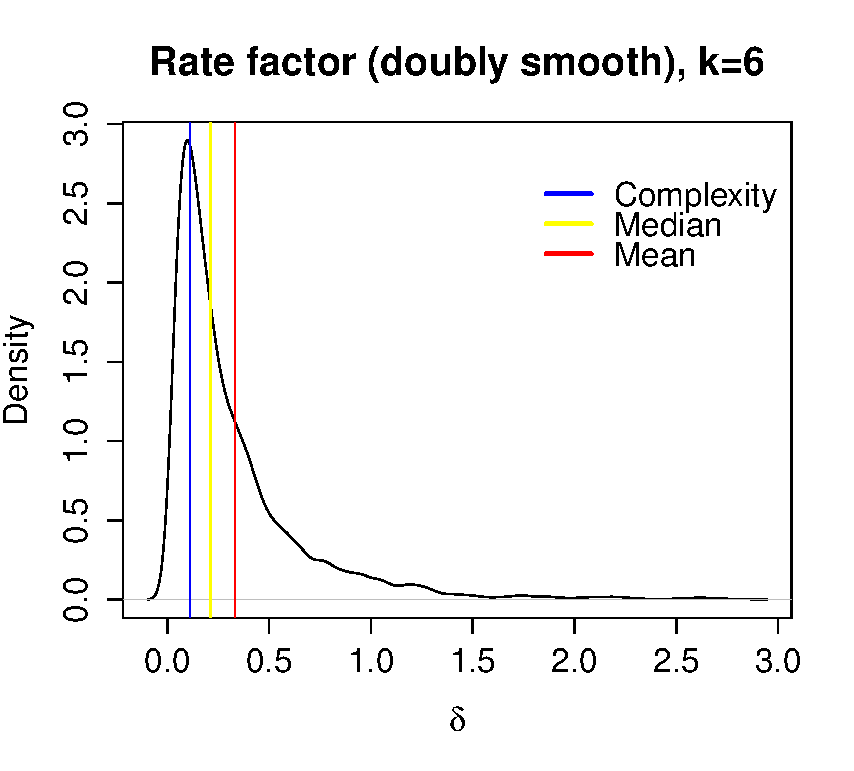
\includegraphics[scale=0.65]{graphs/delta_plot}\label{fig:delta}
\end{center}
Again, as in figure \ref{fig:mults} the value given by the asymptotic complexity is shown, it is indeed the the value which occus with the highest probability. We see again that a much larger proportion of the cases perform significantly better than this case, including the mean case, which the empirical data more closely reflects. We reach the same conclusion that the complexity analysis gives a misleading estimate of the average case.

\end{document}

